\documentclass[12pt,a4paper]{report}
\usepackage[utf8]{inputenc}
\usepackage{graphicx}
\graphicspath{ {C:/Users/kamila/Documents/Praca licencjacka/} }
\usepackage{amsmath}
\usepackage{amsfonts}
\usepackage{amssymb}
\usepackage{amsthm}
\usepackage{paralist}
\usepackage{polski}
\usepackage[hidelinks]{hyperref}
\usepackage{natbib} % potrzba do bibliografii
\usepackage[left=2cm,right=2cm,top=2cm,bottom=2cm]{geometry}
%\usepackage[acronym]{glossaries} COS NIE DZIALA WYWALA BLEDY

\author{Kamila Choja}
\title{Wybrane zastosowanie statystycznych metod porządkowania danych wielowymiarowych}


\newtheorem{theorem}{Twierdzenie}[section]
\newtheorem{definition}[theorem]{Definicja}
\newtheorem{uwaga}{Uwaga}
\newtheorem{example}{Przykład}
\newtheorem{stwierdzenie}{Stwierdzenie}
\newtheorem{wlasnosci}{Własności}

\newcommand{\setR}{\mathbb{R}}

\newcommand{\Lp}[2]{\operatorname{L}_{#1} \left( {#2} \right)}
\newcommand{\norm}[2][]{\left\| {#2} \right\|_{#1}}
\newcommand{\distance}[3][d]{\operatorname{#1}\left( {#2}; {#3}\right)}
\newcommand{\mediana}{\operatorname{med}}

\newcommand{\closure}[1]{\overline{#1}}
\begin{document}
\begin{titlepage}
\begin{center}
        \vspace*{1cm}
        {\large POLITECHNIKA ŁÓDZKA}\\
       \vspace*{1cm}
        {\large WYDZIAŁ FIZYKI TECHNICZNEJ, INFORMATYKI I MATEMATYKI STOSOWANEJ}\\
        \vspace*{2cm}
    \end{center}        
        
\text{Kierunek: Matematyka}\\
\vspace*{0.3cm}
\hspace*{0.3cm}
\text{Specjalność: Matematyczne Metody Analizy Danych Biznesowych}
  
\begin{center}
\rule{\textwidth}{0.5pt}

\vspace*{0.5cm}
   
{\large WYBRANE ZASTOSOWANIE STATYSTYCZNYCH METOD\\ }
{\large PORZĄDKOWANIA DANYCH WIELOWYMIAROWYCH\\}
\vspace*{1cm}


\begin{flushright}
Kamila Choja\\
Nr albumu: 204052 
 \end{flushright}
\rule{\textwidth}{0.5pt}

Praca licencjacka\\
napisana w Instytucie Matematyki Politechniki Łódzkiej\\

\vspace*{2cm}

Promotor: dr, mgr inż. Piotr Kowalski\\
\vfill
ŁÓDŹ, xxx 2018


     \end{center}   
\end{titlepage}

\tableofcontents

\chapter{Wstęp}


\chapter{Preliminaria}  

\section{Notacja} 
\noindent

Poniżej znajduje się lista pojęć powszechnie używanych w pracy wraz z symbolami, które im się przypisuje. 
  
\begin{itemize}
\item $\mathbb{R}$ - zbiór liczb rzeczywistych
\item $\mathbb{N}$ - zbiór liczb naturalnych
%+-\item $\mathcal{E}^n$ - przestrzeń euklidesowa n-wymiarowa
\item O = $\{$O$_{1}$, O$_{2}$, ..., O$_{n}\}$ - zbiór obiektów przestrzennych, $n \in \mathbb{N}$
\item X = $\{$X$_{1}$, X$_{2}$, ..., X$_{n}\}$ - zbiór zmiennych (cech), gdzie $n \in \mathbb{N}$
%\item T = $\{$T$_{1}$, T$_{2}$, ..., T$_{k}\}$ - zbiór okresów (jednostek czasu)
%\item OX = O $\cdot$ X - zbiór obiekto-zmiennych 
%\item OT = O $\cdot$ T - zbiór obiekto-okresów
%\item XT = X $\cdot$ T - zbiór zmienno-okresów
%\item OXT = O $\cdot$ X $\cdot$ T - zbiór obiekto-zmienno-okresów
\item $\Omega$ - przestrzeń zdarzeń elementarnych
\item $\omega$ - zdarzenie elementarne 
\item $\mathcal{F}$ - rodzina podzbiorów zbioru $\Omega$
\item $\sigma$ -  sigma ciało zbiorów $\mathcal{F}$
\item $\mathcal{B}$ - rodzina zbirów borelowskich
\item $\mathfrak{B}$ -rodzina wszystkich zbiorów otwartych %https://www.sharelatex.com/learn/Mathematical_fonts
\item $\mediana (X_{j})$ - mediana cechy $X_{j}$
\item $\rho$ - relacja porządkująca
\item $G$ - graf prosty
\item $V(G)$ - zbiór wierzchołków grafu $G$
\item $E(G)$ - krawędzie grafu $G$
%\item $D$ - graf skierowany(digraf)
%\item $V(D)$ - zbiór wierzchołków digrafu $D$
%\item $A(D)$ - rodzina łuków digrafu $D$


\end{itemize}
\newpage

\section{Słownik użytych pojęć}
W pracy zostały wykorzystane następujące pojęcia, których wytłumaczenie znajduje się poniżej. 
\begin{itemize}
%pojecia proby,statystyi, modelu - formalne mozna podac w oparciu o wyklady Bartoszewicza i pliku- "proba_mod staty_statytsyka folder: pliki pdf do pracy
\item Statystyka matematyczna \cite[w oparciu o rozdział 1]{gren1}\\
Statystyka matematyczna zajmuje się metodami wnioskowania o całej zbiorowości statystycznej na podstawie zbadania pewnej jej części zwanej próbką lub próbą.\\

\item Model statystyczny \cite[w oparciu o rozdział 2]{bartoszewicz1996}\\
Modelem statystycznym nazywamy przestrzeń próby doświadczenia tj. wartości zmiennych losowych o jednakowym rozkładzie, rodzinę podzbiorów zbioru zmiennych oraz prawdopodobieństwo występowania danej zmiennej. Można tutaj wskazać analogię do rachunku prawdopodobieństwa, tj. uporządkowanej trójki $(\Omega,\mathcal{F},P)$.
 
\item Cecha statystyczna \cite[Rozdział 1]{mlodak2006}\\
Cecha statystyczna jest to liczbowy opis przedmiotu dociekań tj. konkretnej dziedziny życia społeczno-gospodarczego.Służy ona do scharakteryzowania podmiotu badania.\\

%mozliwa modyfikacja definicji na przedstawieniu macierzy jako funkcji
\begin{definition}{Macierz \cite[w oparciu o rozdział 1.1]{banaszak2002}\\}
Niech $X$ będzie skończonym podzbiorem liczb $\mathbb{R}$. Macierzą wymiaru $m\times n$ (tzn. o $m$ wierszach i $n$ kolumnach) nazywamy prostokątną tablicę utworzoną z elementów zbioru $X$, postaci:
\begin{center}
$$X= \left[
        \begin{array}{ccccc}
a_{11} & a_{12} & ... & a_{1n}\\
a_{21} & a_{22} & ... & a_{2n}\\
$...$ & $...$ & $...$ & $...$\\
a_{m1} & a_{m2} & ... & a_{mn}
         \end{array}
     \right] $$
\end{center}
gdzie:
\\* $a_{ij} \in X$, dla $ 1 \leq i\leq m, \quad 1\leq j \leq n$
\end{definition}

\item Macierz obserwacji \cite[Rozdział 2]{mlodak2006}\\
Niech $m>1$ oraz $n>1$ będą liczbami naturalnymi.  Macierzą obserwacji nazywamy macierz rozmiaru  $n \times m$  postaci
\begin{center}

$$X= \left[
        \begin{array}{ccccc}
x_{11} & x_{12} & ... & x_{1m}\\
x_{21} & x_{22} & ... & x_{2m}\\
$...$ & $...$ & $...$ & $...$\\
x_{n1} & x_{n2} & ... & x_{nm}
         \end{array}
     \right] $$
\end{center}
gdzie:
\\* $x_{ij}$ - zaobserwowana wartość $j$-tej cechy dla $i$-tego obiektu .\\

\begin{definition}{Macierz odległości zmiennych \cite[Rozdział 1.6]{panek2013}\\}
Macierzą odległości cech zmiennych nazywamy macierz, której elementami są odległości między parami badanych obiektów: 
\begin{center}
$D = [d_{ii'}].$\\
\end{center}
gdzie:\\
$dii'$-odległość między $i$-tym a $i'$-tym obiektem, dla $i,i'=1,2,...,n$
\end{definition}

\item Skala \cite[w oparciu o rozdział 1.2]{panek2013}\\
Skalą nazywamy pewien skończony zbiór, umożliwiający porównywanie obiektów na podstawie wartości  lub własności wybranych zmiennych.

\item Skala porządkowa \cite[Rozdział 1.2]{panek2013}\\
Skala ta pozwala na stwierdzeniu o identyczności lub różnicy porównywanych obiektów, a także na porównywanie wariantów cech zaobserwowanych w obiektach. Nie pozwala ona określić odległości między obiektami. Umożliwia zliczanie obiektów uporządkowanych (liczby relacji równości, nierówności, większości i mniejszości). Przykład zmiennych przedstawianych na skali porządkowej: wykształcenie, kolejność zawodników na podium, oceny w systemie szkolnym.\\

\item Skala przedziałowa \cite[Rozdział 1.2]{panek2013}\\
Jest to skala, która w stosunku do skali porządkowej, pozwala obliczyć odległość między obiektami, dokonując pomiaru cech za pomocą liczb rzeczywistych. Dla skali tej możliwe jest korzystanie z operacji dodawania oraz odejmowania. Dla skali tej istnieje charakterystyczna wartość - punkt zerowy. Jest on wyznaczany w sposób umowny, umożliwia on do zachowania różnic między wartościami cechy, przy zmianie jednostek miary. Przykład zmiennych przedstawianych na skali przedziałowej: temperatura, rok urodzenia.\\ %Wartość zerowa na tej skali ma charakter umowny, co prowadzi do zachowania różnic między wartościami cechy, przy zmianie jednostek miary. \\

\item Skala ilorazowa \cite[Rozdział 1.2]{panek2013}\\
Skala ta, podobna jest do skali przedziałowej, z tym że występuje w niej zero bezwględne - punkt, który mówi o tym, że dana zmienna nie występuje, oraz ogranicza lewostronnie zakres skali ilorazowej. Powoduje to, że można na tej skali obok operacji dodawania i odejmowania, dokonywać także dzielenia i mnożenia, a tym samym przedstawiać dowolną wartość cechy danego obiektu jako wielokrotność wartości cechy dla innego obiektu. Przykład zmiennych przedstawianych na skali ilorazowej: napięcie elektryczne, bezrobocie, inflacja.\\

%\item Zmienna objaśniająca \cite[Rozdział 1.1] {grabinski1982}
%Zmienną objaśniającą nazywamy zmienną w modelu statystycznym, która oddziałuje na zmienne objaśniane. Zmiennie  %objaśniającą oznaczamy jako $X_{1}, ..., X_{k}$, z kolei zmienne objaśniane jako $Y$. \\

\item Stymulanta \cite[Rozdział 1.5]{panek2013}\\
Stymulantami nazywane są zmienne, których wysokie wartości badany w badanych obiektach są pożądane z punktu widzenia rozpatrywanego zjawiska.\\

\item Destymulanta \cite[Rozdział 1.5]{panek2013}\\
Destymulantami nazywane są zmienne, których wysokie wartości badany w badanych obiektach są niepożadane z punktu widzenia rozpatrywanego zjawiska.\\

\item Nominanta \cite[Rozdział 1.5]{panek2013}\\
Nominantami nazywane są zmienne, których odchylenia wartości w badanym obiekcie od wartości (lub przedziału wartości) uznawanych za najkorzystniejsze są niepożądane z punktu widzenia rozpatrywanego zjawiska.\\

%\item Transformacja normalizacyjna \cite[Rozdział 1.5]{panek2013}\\
%Transformacją zmiennych diagnostycznych, mających na celu ujednolicenie ich jednostek pomiarowych, przy zastosowaniu zmiennych diagnostycznych, nazywana jest transformacją normalizacyjną. Można ją przeprowadzić na zmiennych, opisujących porównywane obiekty, mierzonych na skali przedziałowej lub ilorazowej.\\ 
%\\*Ogólny wzór na przekształcenie normalizacyjne(Borys, 1978; Grabiński i in., 1989):
%\begin{center}
%\begin{equation}
%z_{ij}=\left(\frac{x_{ij} - a}{b}\right)^p , i=1,2,...,n; j=1,2,...,m; b\neq0,
%\end{equation}\\
%\end{center}
%gdzie:
%\\* $z_{ij}$ - znormalizowana wartość $j$-tej zmiennej w $i$-tym obiekcie,
%\\* $a,b,p$ - parametry normalizacyjne.

%\item Stopień podobieństwa obiektów \cite[Rozdział 1.6]{panek2013}\\
%Stopień podobieństwa obiektów, jest wielkość mówiąca o podobieństwie obiektów między sobą. Jest on mierzony za pomocą miar odległości lub tez miar bliskości(zgodności).\\

%\item Miara odległości \cite[Rozdział 1.6]{panek2013}\\
%Miarą odległości pomiędzy obiektami: $i$-tym i $i'$-tym, nazywamy dowolną funkcję rzeczywista $d$, spełniającą następujące %warunki:\\
%- {\bf dodatniość} (odległość między różnymi obiektami jest zawsze dodatnia): $d_{ii'}>0$\\
%- {\bf symetryczność} (odległość $i$-tego obiektu od $i'$-tego obiektu jest taka sama, jak odległość $i'$-tego obiektu od 		obiektu $i$-tego: $d_{ii'}=d_{i'i}$\\
%- {\bf zwrotność} (odległość obiektu od samego siebie jest równa zeru): $d_{ii}=0$\\
%- {\bf nierówność trójkąta}: odległość pomiędzy $i$-tym i $i'$-tym obiektem będzie nie większa niż odległość pośrednia pomiędzy tymi obiektami definiowana jako suma odległości pomiędzy obiektami $i$-tym i $i''$-tym oraz $i'$-tym i $i''$-tym): $d_{ii'} \leq d_{ii''} + d_{i''i'}$.\\

%\begin{uwaga}
%Wzrost wartości miary odległości oznacza zmniejszenie stopnia podobieństwa obiektów.\\
%\end{uwaga}

%\item Odległość euklidesowa dla znormalizowanych zmiennych \cite[Rozdział 1.6]{panek2013}\\
%Wzór odległości euklidesowej, dla znormalizowanych zmiennych, jest następujący:
%\begin{center}
%$$d_{ii'}=\big[\sum_{j=1}^{m}|z_{ij}-z_{i'j}|^{2} \big]^{\frac{1}{2}}$$
%\end{center}

%\item Odległość miejska(Manhattan) dla znormalizowanych zmiennych \cite[Rozdział 1.6]{panek2013}\\
%Wzór na odległość miejską(Manhattan) dla znormalizowanych zmiennych, jest następujący:
%\begin{center}
%$$d_{ii'}=\sum_{j=1}^{m}|z_{ij}-z_{i'j}|.$$
%\end{center}

%\item Miara bliskości \cite[Rozdział 1.6]{panek2013}\\
%Miarą bliskości pomiędzy obiektami, nazywamy funkcję $p$ spełniającą następujące warunki:\\
%- {\bf dodatniość}: $p_{ii'} > 0$,\\
%- {\bf symetryczność}: $p_{ii'} = p_{i'i}$\\
%- {\bf zwrotność}: $p_{ii} = 1$.\\
%: Wzrost wartości miary bliskości oznacza zwiększenie stopnia podobieństwa badanych obiektów.\\

%\item Macierz odległości \cite[Rozdział 1.6]{panek2013}\\
%Macierzą odległości, nazywamy macierz unormowanych danych wejściowych, tj. macierz, której elementami są odległości między %parami badanych obiektów. Macierz odległości jest postaci:
%\begin{center}
%$D = [d_{ii'}], i,i'=1, 2, ..., n.$\\
%\end{center}

%\item Średnia arytmetyczna z próby \cite[Rozdział 2.2]{mlodak2006}\\
%Średnią arytmetyczną wartości cechy $X_{j}$ nazywamy wartość 
%\begin{center}
%$$\overline{x_{j}}= \frac{\sum_{i=1}^{n} x_{ij}}{n}$$\\
%\end{center}

%\item Odchylenie standardowe z próby \cite[Rozdział 2.2]{mlodak2006}\\
%Odchyleniem standardowym cechy $X_{j}$  nazywamy wartość 
%\begin{center}

%$$s_{j}= \sqrt{ s_{j}^2} = \sqrt{\frac{1}{n}\sum_{i=1}^{n} (x_{ij} - \overline{x_{j}})^2}$$\\

%\end{center}

%\item Mediana \cite[Rozdział 2.2]{mlodak2006}\\
%Medianę cechy $X_{j}$ nazywamy wartość \\
%\begin{center}

%med$(X_{j})= 
%y = \left\{ \begin{array}{ll}
%\frac{1}{2}\big(x_{(\frac{n}{2})j} + x_{(\frac{n}{2}+1)j}\big) & \textrm{jeśli n jest parzyste} \\\\
%x_{(\frac{n+1}{2})j} & \textrm{jeśli n jest nieparzyste}\\

%\end{array} \right.
%$\\
%\end{center}

%\item Przestrzeń euklidesowa n-wymiarowa $\mathcal{E}^n$ \citep[Rozdział 9]{kuratowski2004}\\
%Przestrzeń euklidesowa n-wymiarowa, jest przestrzenią metryczną przy zwykłej definicji odległości punktu %$x=(x_1,x_2,...,x_n)$ od punktu $y=(y_1,y_2,...,y_n)$, danej wzorem Pitagorasa
%\begin{center}
%$$|x - y| =\sqrt{\sum_{i=1}^{n} |x_i - y_i|^2}$$
%\end{center}
%gdzie, $x$ i $y$ są ciągami złożonymi z n liczb rzeczywistych.

%\item Obiekt wzorcowy \cite[Rozdział 2.2]{panek2013}\\
%Obiektem wzorcowym nazywany jest obiekt modelowy o pożądanych wartościach zmiennych wejściowych.\\

%\item Obiekt wzorcowy \cite[Rozdział 2.1]{mlodak2006}\\
%Obiektem wzorcowym, nazywamy obiekt powstały na podstawie macierzy wystandaryzowanych zmiennych wejściowych. Współrzędnymi obiektu są: \\
%\begin{center}

%$O_{0}=[z_{0j}], j= 1,2,...,m.$\\

%\end{center}
%gdzie współrzędne obiektu wzorcowego obliczane są na podstawie wzoru:
%\begin{center}
%$z_{oj}=max_{i}$
%\end{center}
%\begin{equation}
%z_{oj}=\left\{ \begin{array}{ll}
%\max\limits_{i} \Big\{z_{ij}\Big\}  & \textrm{dla  } z_{j}^S\\\\
%\min\limits_{i}\Big\{ z_{ij} \Big\} & \textrm{dla } z_{j}^D\\
%\end{array} \right.
%\end{equation}
%gdzie:
%\\*$j=1,2,...,m; i=1,2,...,n.$\\


%\item Funkcja kryterium dobroci uporządkowania \cite[Rozdział 2.2]{panek2013}\\
%Funkcją kryterium dobroci uporządkowania nazywamy funkcję: 
%\begin{center}
%$$F^2= \sum_{i'=1}^{n-1} i' \sum_{i=1}^{n-i'} d_{ii'}$$\\

%\end{center}
%gdzie:
%\\* $d_{i,i'}$ - odległość euklidesowa między $i$-tym i $i'$-tym obiektem . \\



%\begin{definition}{Współczynnik Pearsona \cite[Rozdział 2.2]{mlodak2006}\\}
%Współczynnik Pearsona oznaczamy: 
%\begin{center}
%$r_{jk}= \frac{\mathrm{cov}(X_{j},X_{k})}{s_{j}s_{k}}$\\

%\end{center}
%gdzie:
%\\* $\mathrm{cov}(X_{j},X_{k})$ - kowariancja cech $X_{j}$ i $X_{k}$ .\\
%\end{definition}

%\begin{definition} {Macierz korelacji par zmiennych \cite[Rozdział 2.2]{mlodak2006}\\}
%Macierzą korelacji par zmiennych, nazywamy macierz postaci:
%\begin{center}
%$R= \left[
%        \begin{array}{ccccc}
%1 & r_{12} & ... & r_{1m}\\
%r_{21} & 1 & ... & r_{2m}\\
%$...$ & $...$ & $...$ & $...$\\
%r_{m1} & r_{m2} & ... & 1
%         \end{array}
%     \right] $
%\end{center}
%gdzie:
%\\* $r_{jk}$ - współczynnik korelacji liniowej Pearsona $j$-tej i $k$-tej cechy (czyli $X_{j}$ oraz $X_{k}$) .\\
%\end{definition}
\end{itemize}


\newpage

%% TODO wprowadzic podstawowe pojecia rachunku prawdopodobieństwa
%% TODO wprowadzić przedstrzenie obiektów, cech, czasów oraz macierz obserwacji ''topologia

%% TODO w kolejnej sekcji o porządkach matematycznych

\section{Podstawowe pojęcia rachunku prawdopodobieństwa oraz statystyki}
\noindent

Na potrzeby pracy, zostały wykorzystane pojęcia rachunku prawdopodobieństwa oraz statystyki, konieczne do zrozumienia danych jako próby losowej. W tym celu niezbędne było wprowadzenie definicji prawdopodobieństwa, zmiennej losowej, a także pojęć powiązanych z tymi definicjami tj. ciała zbiorów, $\sigma$-ciała zbiorów, przestrzeni zdarzeń elementarnych, zdarzenia losowego.\\

\begin{definition}{Ciało zbiorów \cite[Rozdział 8.1]{rudnicki2006}\\}
Rodzinę $\mathcal{F}$ podzbiorów, niepustego zbioru $X$ nazywamy ciałem zbiorów, jeżeli spełnia ona następujące warunku: \\
\begin{enumerate}
\item $\emptyset \in \mathcal{F}$,
\item jeżeli $A \in \mathcal{F}$, to $X \setminus A \in \mathcal{F}$,
\item jeżeli $A \in \mathcal{F}$, to $A \cup B \in \mathcal{F}$.\\
\end{enumerate}
\end{definition}

\begin{definition}{$\sigma$-algebra/ciało zbiorów\cite[Rozdział 8.1]{rudnicki2006}\\}
Ciało zbiorów $\mathcal{F}$ nazywamy $\sigma$-ciałem zbiorów, jeżeli spełnia ona warunek
dla dowolnych zbiorów $A_{n} \in \mathcal{F}, n \in \mathbb{N}$, mamy
\begin{center}
$\bigcup\limits_{i=1}^{\infty} A_n \in \mathcal{F}$.
\end{center}
%Elementy $\sigma$-ciała $\mathcal{F}$ nazywamy zbiorami mierzalnymi.\\
\end{definition}

\begin{definition}{Zbiory borelowskie \cite[w opraciu o rozdział 2]{billingsley1987}\\}
Zbiorami borelowskimi względem danej przestrzeni $X$, nazywamy zbiory należące do $\sigma$-ciała $X$ generowanego przez rodzinę $\mathfrak{B}(X)$ - wszystkich zbiorów otwartych w $X$. Rodzinę wszystkich zbiorów borelowskich względem $X$, oznaczamy $\mathcal{B}(X)$.\\
\end{definition}

\begin{definition}{Przestrzeń zdarzeń elementarnych \cite[w oparciu o rozdział 1.1]{krysicki1999}\\}
Zbiór wszyskich możliwych wyników doświadczenia losowego nazywamy przestrzenią zdarzeń elementarnych i oznaczamy przez $\Omega$. Elementy zbioru $\Omega$ nazywamy zdarzeniami elementarnymi i oznaczamy $\omega$.\\
\end{definition}

\begin{definition}{Miara zbioru \cite[Rozdział 2.10] {billingsley1987}\\}
Funkcję $\mu$ określoną na ciele $\mathcal{F}$ podzbiorów zbioru $\Omega$ nazywamy miarą, jeśli spełnia następujące warunki: 
\begin{enumerate}
\item $\mu(A) \in [0, \infty]$ dla każdego zbioru $A \in \mathcal{F}$,
\item $\mu(\emptyset)=0$,
\item jeśli $A_1, A_2,...$ jest ciągiem rozłącznych zbiorów $\mathcal{F}$-mierzalnych takich, że $\bigcup\limits_{k=1}^{\infty} A_k \in \mathcal{F}$, to 
\begin{center}
$$\mu\big(\bigcup\limits_{k=1}^{\infty} A_k\big)=\sum_{k=1}^{\infty} \mu(A_k)$$\\
\end{center}
\end{enumerate}
\end{definition}

\begin{definition}{Przestrzeń mierzalna \cite[Rozdział 2.10]{billingsley1987}\\}
Przestrzenią mierzalną nazywamy parę $(X, \mathcal{F})$, gdzie $\mathcal{F}$ jest $\sigma$-ciałem podzbiorów zbioru $X$\\
\end{definition}

\begin{definition}{Funkcja mierzalna \cite[w oparciu o rozdział 8.2]{rudnicki2006}\\}
Niech $X$ będzie niepustym zbiorem, $\mathcal{F}$  $\sigma$-ciałem na $X$ i $\overline{\mathbb{R}} = \mathbb{R} \cup \{-\infty, \infty \}$. Funkcję $f: X \rightarrow \overline{\mathbb{R}}$ nazywamy mierzalną, jeżeli zbiór
\begin{center}
$\{ x \in X: f(x) > a \}$
\end{center}
jest mierzalny przy dowolnym $a \in \mathbb{R}$.\\
\end{definition}

\begin{definition}{Zdarzenie losowe \cite[w oparciu o rozdział 1.1]{krysicki1999}\\}
Zdarzeniem losowym (zdarzeniem) nazywamy każdy podzbiór $\textit{A}$ zbioru $\Omega$, taki że  $A \in \mathcal{F}$, gdzie $\mathcal{F}$ jest rodziną podzbiorów $\Omega$ spełniającą następujące warunki:
\begin{enumerate}
\item $\Omega \in \mathcal{F}$;
\item Jeśli $A \in \mathcal{F}$, to $\textit{A$'$} \in \mathcal{F}$, gdzie $\textit{A$'$} = \Omega \setminus A $ jest zdarzeniem przeciwnym do zdarzenia $\textit{A}$;
\item Jeśli $\textit{A}_{i} \in \mathcal{F}$, $i= 1, 2, ...$,to $\bigcup\limits_{i=1}^{\infty} A_{i} \in \mathcal{F} $
\end{enumerate}
Rodzinę $\mathcal{F}$ spełniającą warunki 1 - 3 nazywamy $\sigma$-ciałem podzbiorów zbioru $\Omega$\\
\end{definition}

\begin{definition}{Prawdopodobieństwo \cite[w oparciu o rozdział 1.1]{krysicki1999}\\}
Prawdopodobieństwem nazywamy dowolną funkcję $P$ o wartościach rzeczywistych, określoną na $\sigma$-ciele zdarzeń $\mathcal{F} \subset 2^\Omega$, spełniającą warunki: \\
\begin{enumerate}
\item $\textit{P(A)} \geq 0 \quad \forall{\textit{A} \in \mathcal{F}}$
\item $\textit{P}(\Omega) = 1$
\item Jeśli $\textit{A}_{i} \in \mathcal{F}$, $i= 1, 2, ...$ oraz $A_{i} \cap A_{j}$ dla $i \neq j$, to 
\end{enumerate}
\begin{center}
$$P \Big(\bigcup\limits_{i=1}^{\infty} A_{i} \Big)=\sum_{i=1}^{\infty} P(A_{i}) $$\\
\end{center}
\end{definition}


\begin{definition}{Przestrzeń probabilistyczna \cite[w oparciu o rozdział 1.2]{krysicki1999}\\}
Przestrzenią probabilistyczną nazywamy uporządkowaną trójkę $(\Omega, \mathcal{F}, P)$, gdzie $\Omega$ jest zbiorem zdarzeń elementarnych, $\mathcal{F}$ jest $\sigma$-ciałem podzbiorów $\Omega$, zaś $P$ jest prawdopodobieństwem określonym na $\mathcal{F}$.\\
\end{definition}

%\begin{definition}{Przestrzeń mierzalna w n-wymiarowej przestrzeni euklidesowej \cite[Rozdział 1]{bartoszewicz1996}\\}
%Niech $(\Omega, \mathcal{F}, P)$ oznacza przestrzeń probabilistyczną. Przestrzenią mierzalną w n-wymiarowej przestrzeni euklidesowej $R^n$, nazywamy uporządkowaną dwójkę $(R^n, \textit{B}^n)$, gdzie $\textit{B}^n$ jest $\sigma$-ciałem podzbiorów borelowskich tej przestrzeni, $n \geq 1$. \\
%\end{definition}



\begin{definition}{Zmienna losowa \cite[Rozdział 2.1]{krysicki1999}\\}
Niech $(\Omega, \mathcal{F}, P)$ będzie dowolną przestrzenią probabilistyczną. Dowolną funkcję $\textit{X} : \Omega \rightarrow \mathbb{R}$ nazywamy zmienną losową jednowymiarową, jeśli dla dowolnej liczby rzeczywistej $x$ zbiór zdarzeń elementarnych $\omega$, dla których spełniona jest nierówność $X(\omega)< x$ jest zdarzeniem, czyli 
\begin{center}
$\{\omega: X(\omega) < x \} \in \mathcal{F}$ dla każdego $x \in \mathbb{R}$\\
\end{center}
\end{definition}

\begin{definition}{Wektor losowy \cite[Rozdział 5.1]{jakubowski2004}\\}
Wektorem losowym nazywamy odwzorowanie $X:\Omega \rightarrow \mathbb{R}^n$, spełniające następujący warunek: dla każdego układu liczb $t_1,t_2,...,t_n \in \mathbb{R}^n$ zbiór $X^{-1}((-\infty,t_1]\times...\times(-\infty,t_n])$ należy do $\mathcal{F}$.\\
\end{definition}

\begin{definition}{Rozkład prawdopodobieństwa zmiennej losowej X \cite[Rozdział 5.1]{jakubowski2004}\\}
Rozkładem prawdopodobieństwa zmiennej losowej o wartościach w $\mathbb{R}$ nazywamy funkcję $\mu_X$ określoną na $\mathcal{B}(\mathbb{R})$ zależnością
\begin{center}
$\mu_X(B)=P_X(B)=P(X^{-1}(B)), \quad B \in \mathcal{B}(\mathbb{R})$\\
\end{center} 
\end{definition}

\begin{definition}{Rozkład dyskretny \cite[Rozdział 5.1]{jakubowski2004}\\}
Mówimy, że zmienna losowa $X$ ma rozkład dyskretny, jeśli istnieje przeliczany zbiór $S \in \mathbb{R}$, taki że $\mu_X(S)=1$.\\
\end{definition}

\begin{definition}{Gęstość i rozkład ciągły \cite[Rozdział 5.1]{jakubowski2004}\\}
Jeśli $\mu$ jest rozkładem prawdopodobieństwa na $\mathbb{R}$ i istnieje całkowalna funkcja $f: \mathbb{R} \rightarrow \mathbb{R}$ taka, że 
\begin{center}
$$\mu(A)=\int_A f(x)dx,   A\in \mathcal{B}(\mathbb{R})  $$  %\quad dla \quad wszystkich
\end{center}
to funkcję $f$ nazywamy gęstością rozkładu $\mu$. Rozkład który ma gęstość, nazywamy rozkładem ciągłym. \\
\end{definition}

%\begin{definition}{Wektor losowy n-wymiarowy \cite[Rozdział 1]{bartoszewicz1996}\\}
%Wektorem losowym n-wymiarowym nazywamy funkcję $X: \Omega \rightarrow \mathbb{R}^n$ mierzalną względem $\sigma$-ciała $\mathcal{F}$ ($\mathcal{F}$-mierzalną), tzn. taką, że $X^{-1}(B) \in \mathcal{F}$ dla każdego $B \in \mathfrak{B}^n$.\\
%\end{definition}

\begin{definition}{Wartość oczekiwana \cite[Rozdział 2.6]{krysicki1999}\\}
Niech $X$ będzie zmienną losową typu dyskretnego lub ciągłego. Wartością oczekiwaną zmiennej losowej $X$ nazywamy 
\begin{center}
$$\displaystyle \mathrm{E}(X)=\mu_X=\left\{ \begin{array}{ll}
\sum\limits_{i=1}^{n} {x_ip_i}, & \textrm{jeśli zmienna ma rozkład dyskretny} \\\\
\int\limits_{-\infty}^{\infty} {xf(x)dx}, & \textrm{jeśli zmienna ma rozkład ciągły}\\
\end{array} \right.$$\\
\end{center}
\end{definition}

\begin{definition}{Wariancja \cite [Rozdział5.6]{jakubowski2004}\\}
Niech $X$ będzie zmienną losową o skończonej wartości oczekiwanej tj. $\mathrm{E}|X| < \infty$. Wariancją zmiennej losowej $X$ nazywamy liczbę
\begin{center}
$VarX= \mathcal{D}^2X=\mathrm{E}(X-\mathrm{E}X)^2$.\\
\end{center}
W przypadku zmiennej losowej o rozkładzie dyskretnym lub ciągłym mamy
\begin{center}
$$\displaystyle VarX=\left\{ \begin{array}{ll}
\sum\limits_{i=1}^{n} (x_i-\mu_X)p_i=\sum\limits_{i=1}^{n} x_{i}^2p_i-(\mu_X)^2, & \textrm{jeśli zmienna ma rozkład dyskretny} \\\\
\int\limits_{-\infty}^{\infty}(x-\mu_X)^2f(x)dx=\int\limits_{-\infty}^{\infty} x^{2}f(x)dx-(\mu_X)^2, & \textrm{jeśli zmienna ma rozkład ciągły}\\
\end{array} \right.$$\\
\end{center}
\end{definition}


\begin{definition}{Odchylenie standardowe \cite[Rozdział 5.6]{jakubowski2004}\\}
Niech $X$ będzie zmienną losową. Odchyleniem standardowym nazywamy pierwiastek z wariancji. 
\begin{center}
$\sigma_X=\sqrt{\mathcal{D}^2X}$\\
\end{center}
\end{definition}

\begin{definition}{Rozkład normalny (Gaussa) \cite[Rozdział 5.10]{jakubowski2004}\\}
Jeśli zmienna losowa $X$ ma gęstość postaci
\begin{center}
$f(x)=\frac{1}{\sqrt{2\pi}\sigma}e^\frac{-(x-\mu_X)^2}{2\sigma^2}$ 
\end{center}
dla $x \in \mathbb{R}$ i pewnych $\mu_X \in \mathbb{R}$ i $\sigma^2 >0$. To mówimy, że zmienna losowa ma rozkład normalny z parametrami $\mu$ i $\sigma^2$, co zapisujemy $\mathcal{N}(\mu, \sigma^2)$.\\
W przypadku, gdy $\mu=0$ i $\sigma^2=1$, to rozkład ten nazywamy standardowym rozkładem normalnym i oznaczamy $\mathcal{N}(0,1)$, a gęstość jest postaci
\begin{center}
$f(x)=\frac{1}{\sqrt{2\pi}}e^\frac{-(x)^2}{2}.$ 
\end{center}
\end{definition}

%\begin{definition}{Wartość oczekiwana macierzy losowej $X$ \cite[Rozdział 1.3]{bartoszewicz1996}\\}
%Wartością oczekiwaną macierzy losowej $X$ nazywamy macierz postaci:
%\begin{center}
%$\mathrm{E}(X)=\left[
%       \begin{array}{ccccc}
%\mathrm{E}(X_{11}) & \mathrm{E}(X_{12}) & ... & \mathrm{E}(X_{1r})\\
%\mathrm{E}(X_{21}) & \mathrm{E}(X_{22}) & ... & \mathrm{E}(X_{2r})\\
%$...$ & $...$ & $...$ & $...$\\
%\mathrm{E}(X_{n1})& \mathrm{E}(X_{n2}) & ... & \mathrm{E}(X_{nr})
%         \end{array}
%     \right] $\
%\end{center}
%przy założeniu, że wszystkie wartości oczekiwane $\mathrm{E}(X_{ij})$, $i=1, 2, ..., n, j=1, 2, ..., r$, istnieją.\\
%\end{definition}

%\begin{definition}{Macierz kowariancji n-wymiarowego wektora losowego $X$ \cite[Rozdział 1]{bartoszewicz1996}\\}
%Macierzą kowariancji n-wymiarowego wektora losowego $X$ nazywamy macierz
%\begin{center}
%$\sum=\mathrm{E}\{[X-\mathrm{E}(X)][X-\mathrm{E}(X)]'\}$\\
%\end{center}
%\end{definition}

%\begin{definition}{Kowariancja \cite[Rozdział 1]{bartoszewicz1996}\\}
%Niech $X_{i}$ i $X_{j}$ będą zmiennymi losowymi, $\sum$ będzie macierzą kowariancji n-wymiarowego wektora losowego $X$. Kowariancją zmiennych losowych $X_{i}$ i $X_{j}$, nazywamy 
%\begin{center}
%$\mathrm{cov}(X_{i},X_{j})=\sigma_{ij}=\mathrm{E}\{[X_{i}-\mathrm{E}(X_{i})][X_{j}-\mathrm{E}(X_{j})]\}$, $i, j= 1, 2, ..., n$
%\end{center}
%gdzie $\sigma_{ij}$ jest elementem macierzy kowariancji n-wymiarowego wektora losowego $X$.\\
%\end{definition}



\newpage
\section{Podstawowe pojęcia teorii grafów} %https://edu.pjwstk.edu.pl/wyklady/mad/scb/mad03/main03_p1.html
\noindent

W pracy zostaną opisane zarówno metody porządkowania liniowego jak i nieliniowego tzn. w ujęciu matematycznym - porządku częściowego, w tym celu należy wprowadzić definicje związane z teorią grafów, niezbędne przy opisywaniu metod porządkowania nieliniowego.

W celu wprowadzeniu złożonych definicji, należy wcześniej podać podstawowe pojęcia dotyczące grafów. Uprzednio zostanie jeszcze wprowadzona definicja pary uporządkowanej oraz nieuporządkowanej, gdyż pojęcia te zostały wykorzystane w definicji grafu.
%Poniższe pojęcia zostały opracowane na podstawie \cite{wilson2008}\\

%grafika grafu z wierzchołkami zastanowic sie  https://www.sharelatex.com/learn/Inserting_Images
%make glossary do wprowadzenia pojec -> poczytac i sie zastanowic


\begin{definition}{Para uporządkowana \cite[w oparciu o rozdział 3]{kuratowski2004}\\}
Niech dane będą dwa elementy $a$ i $b$. Parą uporządkowaną nazywamy parę postaci $<a,b>$, gdzie element $a$ jest poprzednikiem, zaś element $b$ jest następnikiem. 
\begin{center}
$<a,b>=\{\{a\},\{a,b\}\}$.
\end{center}
\end{definition}

\begin{definition}{Para nieuporządkowana \cite[w oparciu o rozdział 3]{kuratowski2004}\\}
Niech dane będą dwa elementy $a$ i $b$. Parą nieuporządkowaną nazywamy zbiór postaci $\{a,b\}$, zawierający elementy $a$ i $b$ i nie zawierający żadnego innego elementu. W przypadku, gdy $a=b$, to para nieuporządkowana $\{a,b\}$, składa się dokładnie z jednego elementu.

\end{definition}


\begin{definition}{Graf \cite[w oparciu o rozdział 2]{wilson2008}\\}
Grafem nazywamy parę $G=(V,E)=(V(G),E(G))$, gdzie $V$ jest niepustym, skończonym zbiorem wierzchołków grafu $G$, zaś $E$ jest skończonym podzbiorem zbioru nieuporządkowanych par elementów zbioru $V$.
%Niech $G$ będzie grafem, tzn. zbiorem składającym się z niepustego, skończonego zbioru $V(G)$, którego elementy nazywamy wierzchołkami oraz skończonego zbioru $E(G)$, którego elementy nazywamy krawędziami. Zbiór $V(G)$ nazywamy zbiorem wierzchołków, a zbiór $E(G)$ zbiorem krawędzi grafu $G$.\
\end{definition}

%\begin{definition}{Graf prosty \cite[Rozdział 2]{wilson2008}\\}
%Niech $G$ będzie grafem prostym, tj. grafem składającym się z niepustego zbioru skończonego $V(G)$, którego elementy nazywamy wierzchołkami (lub węzłami), i skończonego zbioru $E(G)$ różnych par nieuporządkowanych różnych elementów zbioru $V(G)$, które nazywamy krawędziami. Zbiór $V(G)$ nazywamy zbiorem wierzchołków, a zbiór $E(G)$ $\big (E(G) \subseteq \{\{u,v\}: u,v \in V, u\neq v\} \big)$ zbiorem krawędzi grafu $G$.\\
%Mówimy, że krawędź $\{v,w\}$ łączy wierzchołki $v$ i $w$, i na ogół oznaczamy ją krócej symbolem $vw$.\\
%\end{definition}

\begin{definition}{Pętle \cite[Rozdział 2]{wilson2008}\\}
Pętlami nazywamy krawędzie wielokrotne, łączące wierzchołek z samym sobą.\\
\end{definition}

%\begin{definition}{Graf/graf ogólny \cite[Rozdział 2]{wilson2008}\\}
%Grafem nazywamy obiekt, w którym występują krawędzie wielokrotne oraz pętle.\\
%\end{definition}

\begin{definition}{Trasa/marszruta \cite[Rozdział 3]{wilson2008}\\}
Trasą (lub marszrutą) w danym grafie $G$ nazywamy skończony ciąg krawędzi postaci $v_{0}v_{1}, v_{1}v_{2}, ..., \newline v_{m-1}v_{m}$, zapisywany również w postaci $v_{0} \rightarrow{} v_{1} \rightarrow{} v_{2} \rightarrow{} ... \rightarrow{} v_{m}$, w którym każde dwie kolejne krawędzie są albo sąsiednie, albo identyczne. Taka trasa wyznacza ciąg wierzchołków $v_{0}, v_{1}, ..., v_{m}$. Wierzchołek $v_{0}$ nazywamy wierzchołkiem początkowym, a wierzchołek $v_{m}$ wierzchołkiem końcowym trasy; mówimy też wtedy, o trasie od wierzchołka $v_{0}$ do wierzchołka $v_{m}$. Liczbę  krawędzi na trasie nazywamy długością trasy. \\
\end{definition}

\begin{definition}{Ścieżka \cite[Rozdział 3]{wilson2008}\\}
Trasą, w której wszystkie krawędzie są różne, nazywamy ścieżką.\\
\end{definition}

\begin{definition}{Droga \cite[Rozdział 3]{wilson2008}\\}
Ścieżkę, w której wierzchołki $v_{0}, v_{1}, ..., v_{m}$ są różne (z wyjątkiem, być może, równości $v_{0}=v_{m}$), nazywamy drogą. \\
\end{definition}

\begin{definition}{Droga zamknięta/ścieżka zamknięta \cite[Rozdział 3]{wilson2008}\\}
Droga lub ścieżka jest zamknięta, jeśli $v_{0}=v_{m}$.\\
\end{definition}

\begin{definition}{Cykl \cite[Rozdział 3]{wilson2008}\\}
Ścieżką zamkniętą zawierającą co najmniej jedną krawędź nazywamy cyklem. \\
\end{definition}

\begin{definition}{Graf spójny \cite[Rozdział 3]{wilson2008}\\}
Graf jest spójny wtedy i tylko wtedy, gdy każda para wierzchołków jest połączona drogą.\\
\end{definition}
%%ilustracja grafu spójnego

%\begin{definition}{Dendryt \cite[Rozdział 2.3]{panek2013}\\}
%Graf spójny i otwarty nazywany jest dendrytem. \\
%\end{definition}

\begin{definition}{Drzewo \cite[Rozdział 4]{wilson2008}\\}
Drzewem nazywamy graf spójny, nie zawierający cykli.\\
\end{definition}
%dodac grafike drzewa

\begin{definition}{Graf skierowany(digraf albo graf zorientowany) \cite[Rozdział 7]{wilson2008}\\}
Graf skierowany lub digraf $D$, składa się z niepustego zbioru skończonego $V(D)$ elementów nazywanych wierzchołkami i skończonej rodziny $A(D)$ par uporządkowanych elementów zbioru $V(D)$, nazywanych łukami. Zbiór $V(D)$ nazywamy zbiorem wierzchołków, a rodzinę $A(D)$ rodziną łuków digrafu D. Łuk $(v,w)$ zwykle zapisujemy jako $vw$. Graf skierowany oznaczamy zwykle w postaci pary uporządkowanej $G=<V,E>$\\
\end{definition}

\begin{uwaga}
Każdy graf jednoznacznie wyznacza pewną relację dwuargumentową (binarną) w zbiorze $V$. Można również powiedzieć odwrotnie, że każda relacja dwuargumentowa (binarna) $r$ w zbiorze $V$, wyznacza jednoznacznie graf zorientowany, którego węzłami są elementy zbioru $V$, z kolei krawędziami są uporządkowane pary $(v,v^{'})$, należące do $r$. 
\end{uwaga}

\begin{definition}{Graf niezorientowany \cite[Rozdział 2.3]{panek2013}\\}
Grafem niezorientowanym, nazywamy graf $G=<V,E>$, jeżeli relacja binarna tego grafu jest symetryczna, tj. dla dowolnych wierzchołków $v,v^{'} \in V$, $(v,v^{'}) \in E$ wttw $(v^{'},v) \in E$.
\end{definition}

%dodac podstawowe pojecia zwiazane z diagramami, diagramem hessego
\newpage
\section{Wybrane pojęcia z teorii mnogości i topologii: relacja porządkująca, przestrzenie metryczne, miary odległości}
\subsection{Relacja porządkująca}
\noindent

W niniejszej pracy skupiam się na zagadnieniu porządkowania danych wielowymiarowych. Konieczne jest zatem przywołanie odpowiednich sformułowań dotyczących matematycznej definicji porządku. Najbardziej podstawowym pojęciem jest relacja porządku, która zostanie zdefiniowana poniżej. 

%\begin{definition}{Relacja porządkująca \cite[Rozdział 1]{kuratowski2004}\\}
%Niech dana relacja $\rho$, którą oznaczać będziemy przez $\leq$, będzie określona dla elementów ustalonego zbioru $X$. %Mówimy, że relacja $\leq$ jest relacją porządkującą, jeśli spełnione są warunki:
%\begin{enumerate}
%\item $x \leq x$ dla każdego $x$ (zwrotność),
%\item jeśli $x \leq y$ i $y \leq x$, to $x=y$ (symetryczność),
%\item jeśli $x \leq y$ i $y \leq z$, to $x \leq z$ (przechodniość).\\
%\end{enumerate}
%\end{definition}

\begin{definition}{Relacja \cite[Rozdział 3]{kuratowski2004}\\}
Niech dane będą zbiory $X$ i $Y$. Relacją (dwuargumentową) między elementami zbiorów $X$ i $Y$ nazywamy dowolny podzbiór $\rho \subset X \times Y $. Jeśli $X=Y$ to mówimy, że $\rho$ jest relacją na zbiorze $X$. \\
\end{definition} 

\begin{definition}{Relacja porządkująca (częściowego porządku) \cite[Rozdział 2]{blaszczyk2007}\\}
Niech dana relacja $\rho$, którą oznaczać będziemy przez $\leq$, będzie określona dla elementów ustalonego zbioru $X$. Mówimy, że relacja $\leq$ jest relacją częściowego porządku, jeśli spełnione są warunki:
\begin{enumerate}
\item $x \leq x$ dla każdego $x$ (zwrotność),
\item jeśli $x \leq y$ i $y \leq x$, to $x=y$ (słaba antysymetryczność),
\item jeśli $x \leq y$ i $y \leq z$, to $x \leq z$ (przechodniość).\\
\end{enumerate}
\end{definition}


%na podstawie: http://wazniak.mimuw.edu.pl/index.php?title=Matematyka_dyskretna_2/Wyk%C5%82ad_2:
\begin{example}{Częściowego porządku na zbiorze\\}
Wykorzystanie częściowego porządku na płaszczyźnie $\mathbb{R}^2$, obrazuje diagram Hassego, będącego grafem skierowanym, którego wierzchołki zostały poddane relacji porządkowania i reprezentują elementy  skończonego zbioru $X \subset \mathbb{R}$. 
Aby go skonstruować, należy postępować według poniższych kroków:
\begin{itemize}
\item Punkty obrazujące elementy zbioru $X$, umieszcza się na płaszczyźnie.
\item Punkt $x\in X$ łączony jest odcinkiem z punktem $y \in X$, jeśli $x$ jest następnikiem $y$, czyli gdy $y <x$ oraz nie istnieje taki punkt $z \in X$, że $y<z<x$.
\end{itemize}
%moze bez obrazka
%\begin{figure}[h]
%\centering
%\includegraphics[width=1\textwidth]{diagram_hassego}
%\caption{Diagram Hassego}
%\label{fig:obrazek2}
%\end{figure}
\end{example}


\begin{definition}{Relacja liniowo porządkująca (liniowy porządek) \cite[Rozdział 2]{blaszczyk2007}\\}
Niech dany będzie niepusty zbiór $X$. Relację $\leq$ porządkującą zbiór $X$, nazywamy relacją liniowo porządkującą lub porządkiem liniowym, gdy dla dowolnych $x$, $y \in X$ spełnia ona następujący warunek liniowości:
\begin{center}
$x \leq y$ lub $y \leq x$
\end{center}
Parę $(X, \leq)$ nazywamy zbiorem liniowo uporządkowanym lub łańcuchem.\\
\end{definition}

\begin{definition}{Dobry porządek \cite[Rozdział 2]{blaszczyk2007}\\}
Niech dany będzie zbiór $X$. Relację $\leq$ porządkującą zbiór $X$, nazywamy dobrym porządkiem na zbiorze $X$, gdy w każdym niepustym podzbiorze zbioru $X$ istnieje element najmniejszy względem relacji $\leq$. Jeśli relacja $\leq$ na zbiorze $X$ jest dobrym porządkiem, to mówimy, że para $(X,\leq)$ jest zbiorem dobrze uporządkowanym.\\
\end{definition}

\begin{definition}{Ograniczenie górne \cite[Rozdział 2]{blaszczyk2007}\\}
Niech $A \subseteq X$, gdzie $(X, \leq)$ jest zbiorem uporządkowanym. Element $x \in X$ nazywamy ograniczeniem górnym zbioru $A$ względem relacji $\leq$, gdy $a \leq x$ dla każdego $a \in A$. \\
\end{definition}

\begin{definition}{Ograniczenie dolne \cite[Rozdział 2]{blaszczyk2007}\\}
Niech $A \subseteq X$, gdzie $(X, \leq)$ jest zbiorem uporządkowanym. Element $y \in X$ nazywamy ograniczeniem dolnym zbioru $A$ względem relacji $\leq$, gdy $y \leq a$ dla każdego $a \in A$. \\
\end{definition}

\begin{definition}{Zbiór ograniczony z góry, zbiór ograniczony z dołu, zbiór ograniczony \cite[Rozdział 2]{blaszczyk2007}\\}
Niech $A \subseteq X$, gdzie $(X, \leq)$ jest zbiorem uporządkowanym. Zbiór nazywamy ograniczonym z góry (ograniczonym z dołu), jeśli ma on ograniczenie górne (dolne). 
$\newline$ 
Zbiór ograniczony z dołu i z góry nazywamy ograniczonym. \\
\end{definition}

\begin{definition}{Kres górny \cite[Rozdział 2]{blaszczyk2007}\\}
Niech $A \subseteq X$, gdzie $(X, \leq)$ jest zbiorem uporządkowanym. Jeśli zbiór $A$ jest ograniczony z góry i wśród ograniczeń górnych zbioru $A$ istnienie element najmniejszy $x_0$, to element ten nazywamy kresem górnym zbioru $A$ i oznaczamy symbolem $sup A$. Tak więc $x_0 =sup A$, gdy spełnione są następujące warunki:
\begin{enumerate}
\item $a \leq x_0$ dla każdego $a \in A$,
\item jeśli $a \leq x$ dla każdego $a \in A$, to $x_0 \leq x$.
\end{enumerate}
\end{definition}

\begin{definition}{Kres dolnym \cite[Rozdział 2]{blaszczyk2007}\\}
Niech $A \subseteq X$, gdzie $(X, \leq)$ jest zbiorem uporządkowanym. Jeśli zbiór $A$ jest ograniczony z dołu i wśród ograniczeń dolnych zbioru $A$ istnienie element największy $x_0$, to element ten nazywamy kresem dolnym zbioru $A$ i oznaczamy symbolem $inf A$. Tak więc $x_0 =inf A$, gdy spełnione są następujące warunki:
\begin{enumerate}
\item $y_0 \leq a$ dla każdego $a \in A$,
\item jeśli $y \leq a$ dla każdego $a \in A$, to $y \leq y_0$.
\end{enumerate}
\end{definition}

\subsection{Przestrzenie metryczne, miary odległości}
\noindent

Niezbędnym jest również wprowadzenie podstawowych pojęć z topologii, ze względu na stosowanie funkcji odległości w celu uporządkowania obiektów.\\

\begin{definition}{Metryka \cite[Rozdzial 9]{kuratowski2004}\\}
Niech $X$ będzie niepustym zbiorem, wtedy funkcję $\mathrm{d}: X \times X \rightarrow [0,\infty)$, nazywamy metryką jeśli spełnione są warunki:
\begin{enumerate}
\item $\forall x, y \in X \quad \big(\mathrm{d}(x,y) = 0  \Longleftrightarrow x=y \big)$,
\item $\forall x, y \in X \quad \mathrm{d}(x,y)=\mathrm{d}(y,x)$,
\item $\forall  x, y, z \in X \quad \mathrm{d}(x,y)\leq \mathrm{d}(x,z)+\mathrm{d}(z,y)$.\\
\end{enumerate}
%Parę $\(X,\mathrm{d})$ nazywamy przestrzenią metryczną.
\end{definition}

\begin{definition}{Przestrzeń metryczna \cite[Rozdział 9]{kuratowski2004}\\}
Niech $X$ będzie niepustym zbiorem, $\mathrm{d}$ metryką, wówczas parę $(X,\mathrm{d})$ nazywamy przestrzenią metryczną. \\
\end{definition}

\begin{example}{Metryka euklidesowa w $\mathbb{R}^2$}\\
Niech $\mathrm{d}_e: \mathbb{R}^2 \times \mathbb{R}^2 \rightarrow \mathbb{R}$ będzie metryką euklidesową, wówczas \\$\forall{(x_{1},x_{2}),(y_{1},y_{2}) \in \mathbb{R}^2} \quad \mathrm{d}_e((x_1,y_1),(x_2,y_2)):= \sqrt{(x_2-x_1)^2+(y_2-y_1)^2}. $
%Niech $x=(x_1,x_2)$ oraz $y=(y_1,y_2)$, wówczas 
%\begin{center}
%$\mathrm{d}_e((x_1,y_1),(x_2,y_2)):= \sqrt{(x_2-x_1)^2+(y_2-y_1)^2}.$\\
%\end{center}
\end{example}

\begin{example}{Metryka miejska(Manhattan) w $\mathbb{R}^2$}\\
Niech $\mathrm{d}_m: \mathbb{R}^2 \times \mathbb{R}^2 \rightarrow \mathbb{R}$ będzie metryką miejską, wówczas \\
%\begin{center}
$\forall{(x_{1},x_{2}),(y_{1},y_{2}) \in \mathbb{R}^2} \quad \mathrm{d}_m((x_1,y_1),(x_2,y_2)):=|x_1-x_2|+|y_1-y_2|.$\\
%\end{center}
\end{example}

\begin{example}{Przestrzeń euklidesowa $n$-wymiarowa $\mathbb{R}^n$\\}
Niech $\mathrm{d}_e: \mathbb{R}^n \times \mathbb{R}^n \rightarrow \mathbb{R}$ będzie metryką euklidesową, wówczas\\   $\forall{(x_1,x_2,...,x_n),(y_1,y_2,...,y_n) \in \mathbb{R}^n} \quad \mathrm{d}_e(x,y):= \sqrt{\sum_{i=1}^{n} |x_i-y_i|^2}.$\
\end{example}

%Tw o metryce euklidesowej w K^n ?? -zeszyt topologia rok 2 


\chapter{Metody porządkowania}
\noindent

Rozdział ten został opracowany w oparciu o \cite[Rozdział 2]{panek2013}, omówiono w nim ogólnie metody porządkowania zarówno liniowego jak i nieliniowego, po to by w kolejnym rozdziale szczegółowo przyjrzeć się wybranym metodą wraz z przedstawieniem ich algorytmów oraz dokładnych opisów matematycznych, z uwzględnieniem ich wad oraz zalet.


Metody porządkowania liniowego pozwalają na ustalenie hierarchii obiektów ze względu na określone kryterium. Z kolei metody porządkowania nieliniowego nie pozwalają na ustaleniu hierarchii, natomiast w wyniku uporządkowania możliwe jest wskazanie dla każdego z obiektów poddanych porządkowaniu, wskazaniu obiektów podobnych ze względu na opisujące je zmienne. 
 %Problematyka związana z grupowaniem obiektów ma tutaj znaczenie drugoplanowe. Natomiast stosowanie metod porządkowania nieliniowego nie pozwala na ustalenie hierarchii obiektów, lecz wyłącznie wskazanie dla każdego z tych obiektów podobnych ze względu na wartości opisujących je zmiennych. Powoduje to, że porządkowanie nieliniowe stanowi przede wszystkim etap wstępny do grupowania obiektów.\\

\section{Metody porządkowania liniowego}
\noindent

Porządkowanie liniowe obiektów polega, w ujęciu geometrycznym, na rzutowaniu na prostą punktów reprezentujących obiekty, umieszczonych w wielowymiarowej przestrzeni zmiennych. Takie postępowanie pozwala na ustalenie hierarchii obiektów, czyli uporządkowanie ich od obiektu stojącego najwyżej w tej hierarchii do obiektu znajdującego się najniżej. Poniżej zostaną przedstawione własności uporządkowania liniowego obiektów, wraz z podaniem matematycznej interpretacji tych własności.\\

\begin{itemize}
\item każdy obiekt ma przynajmniej jednego sąsiada i nie więcej niż dwóch sąsiadów,
\item jeżeli sąsiadem $i$-tego obiektu jest $i'$-ty obiekt, to jednocześnie sąsiadem $i'$-tego obiektu jest $i$-ty obiekt,
\item dokładnie dwa obiekty mają tylko jednego sąsiada.\\
\end{itemize}
\noindent

\begin{definition}{Sąsiad względem relacji $\leq$\\ }
Niech  $X$ będzie niepustym zbiorem, a $x, y$ będą elementami należącymi do tego zbioru. Mówi się, że $y \in X$ jest sąsiadem $x \in X$,co zapisujemy $ySx$, jeśli
\begin{center}
$y \leq x \vee x \leq y \quad \wedge \quad  \lnot \exists_{z \in X} \quad y \leq z \leq x \wedge x \leq z \leq y$.\\
\end{center}
\end{definition}

\begin{wlasnosci}{Porządku liniowego\\}
Niech $\leq$ będzie relacją zdefiniowaną w $X \times X$, taką że:
\begin{enumerate}
\item $\forall_{x \in X} \quad \overline{\overline{\{y \in X, ySx\}}} \in \{1,2\}$,
\item $\forall_{x, y \in X} \quad ySx \Rightarrow xSy $,
%\item $\overline{\overline{\{\x in X, \quad \overline{\overline{\{y \in X, ySx \}=1\}}}}}=2 $
\item $\overline{\overline{\{x \in X, \quad \overline{\overline{\{y \in X, \quad ySx \}}}=1\}}}=2 $
\end{enumerate}
gdzie:\\
$S$ oznacza sąsiada względem relacji $\leq$, z kolei relacja $\leq$ jest porządkiem liniowym zbioru danych $X$.
\end{wlasnosci}

\begin{theorem}{Porządek liniowy zbioru danych $X$ jest porządkiem liniowym w sensie definicji 2.5.3.\\} 
Porządek liniowy zbioru danych $X$ jest porządkiem liniowym w sensie definicji 2.5.3.
\end{theorem}
\begin{proof}
By udowodnić to twierdzenie należy odwołać się do definicji częściowego porządku, a następnie skorzystać z definicji relacji liniowego porządku. Zatem, należy wykazać zwrotność, przechodniość, słabą antysymetryczność oraz spójność relacji. Niech dany będzie skończony, niepusty zbiór $X$ (przez zbiór $X$ będziemy rozumieli zbiór danych), oraz relacja $\leq$.\\
Załóżmy, że zbiór $X \subset \mathbb{R}^2$ oraz $X=\{a_1, a_2,..., a_n\},\quad n\in \mathbb{N}$ oraz $a_i=(x_i,y_i) \in X,  i\in \mathbb{N}$\\
Niech dane będą dwa obiekty $a_i, a_j \in X, \quad a_i=(x_i, y_i)  \wedge a_j=(x_j, y_j),  i, j\in \mathbb{N}$\\
\begin{itemize}%[(alph)]
\item (zwrotność)\\
Zauważmy, że $\forall{a_i \in X}_{i \in \mathbb{N}} \quad a_i \leq a_i$, wtedy
\begin{center}
 $(x_i, y_i) \leq (x_i, y_i)$, czyli $x_i \leq x_i \wedge y_i \leq y_i$. \\
\end{center}
Zatem relacja $\leq$ jest zwrotna.
\item (słaba antysymetryczność)\\
Niech dane będą obiekty $a_i, a_j \in X$ wówczas 
\begin{center}
$a_i \leq a_j \quad \wedge \quad a_j \leq a_i$ czyli\\
$(x_i, y_i) \leq (x_j, y_j) \quad \wedge \quad  (x_j, y_j) \leq (x_i, y_i)$ zatem \\
$(x_i \leq x_j \wedge y_i \leq y_j) \wedge (x_j\leq x_i \wedge y_j \leq y_i)\quad  \Rightarrow \quad x_i=x_j \wedge y_j=y_i \quad \Rightarrow \quad (x_i,y_i)=(x_j,y_j)$
\end{center}
Zatem relacja $\leq$ jest słabo antysymetryczna.
\item (przechodniość)\\
Niech dane będą obiekty $a_i, a_j, a_k \in X$, takie że $\quad a_i \leq a_j \quad  \wedge \quad a_j \leq a_k$
\begin{center}
$(x_i, y_i) \leq (x_j, y_j) \quad \wedge \quad  (x_j, y_j) \leq (x_k, y_k)$ czyli\\ 
$(x_i \leq x_j \wedge y_i \leq y_j) \wedge (x_j \leq x_k \wedge y_j \leq y_k) \quad \Rightarrow$\\
$x_i \leq x_k \wedge y_i \leq y_k \quad \Rightarrow (x_i,y_i) \leq (x_k,y_k)$\\
\end{center}
Zatem $\forall_{a_i, a_j, a_k \in X}\quad a_i \leq a_k,  $ stąd relacja $\leq$ jest przechodnia. 
\end{itemize}
Na podstawie powyższych punktów, widać iż para $(X,\leq)$ jest zbiorem częściowo uporządkowanym, sprawdzimy teraz czy relacja ta jest spójna.
\begin{itemize}
\item (spójność)\\
Niech dane będą obiekty $a_i, a_j \in X$, przy czym $i\neq j, \quad i,j \in \mathbb{N}$.\\
\begin{center}
Wówczas $a_i \leq a_j \vee a_j\leq a_i$, czyli\\
$(x_i,y_i)\leq (x_j,y_j) \quad \vee \quad (x_j,y_j) \leq (x_i, y_i)$\\
$x_i \leq x_j \wedge y_i \leq y_j \quad \quad \vee \quad \quad x_j\leq x_i \wedge y_j\leq y_i$\\
w tym przypadku $a_i \leq a_j \quad  \quad$ z kolei w tym przypadku $a_j \leq a_i.$
\end{center}
W związku z powyższym oznacza to, że obiekty są porównywalne
\end{itemize} 
Wobec powyższych zostało udowodnione, że relacja $\leq$ jest zwrotna, przechodnia, słabo antysymetryczna i spójna, w związku z tym para $(X, \leq)$ jest liniowym porządkiem.


\end{proof}




Aby uporządkować liniowo obiekty, charakteryzujące je zmienne muszą być mierzone przynajmniej na skali porządkowej. Gdy zmienne te mierzone są na skali przedziałowej lub ilorazowej, należy dokonać ich normalizacji, dla zapewnienia ich porównywalności.

Metody porządkowania liniowego można podzielić na metody diagramowe, procedury oparte na zmiennej syntetycznej oraz procedury iteracyjne bazujące funkcji kryterium dobroci uporządkowania tzn. funkcji, którą się przyjmuje, lub też tworzy się ją aby w kolejnych iteracjach szukać takiego uporządkowania, które optymalizuje zbiór wartości tej funkcji. W kolejnej sekcji zostaną pokrótce przedstawione różne metody, z wyszczególnieniem najważniejszych założeniach każdej z nich.

\newpage
\subsection{Metody diagramowe}
\noindent

W metodach diagramowych stosuje się graficzną reprezentację macierzy odległości zwanej diagramem. Macierz konstruowana jest w oparciu o odległości między obiektami, wyznaczone za pomocą dowolnej metryki. Porządkowanie obiektów polega na porządkowaniu diagramu, tj. przestawieniu wierszy i odpowiadających im kolumn diagramu, tak aby symbole graficzne reprezentujące najmniejsze odległości skupiały się wzdłuż głównej przekątnej, zaś w miarę oddalania się od głównej przekątnej znajdowały się symbole graficzne odpowiadające coraz to większym odległością.  %W kolejnym etapie następuje dzielenie mierników odległości macierzy, na klasy podobieństwa obiektów. Kolejny krok polega na przyporządkowaniu poszczególnym klasom podobieństwa, obiektów odpowiedniego symbolu graficznego. Samo porządkowanie obiektów polega na porządkowaniu diagramu, tj. przestawieniu wierszy i odpowiadających im kolumn diagramu, tak aby symbole graficzne reprezentujące najmniejsze odległości skupiały się wzdłuż głównej przekątnej, zaś w miarę oddalania się od głównej przekątnej znajdowały się symbole graficzne odpowiadające coraz to większym odległością. 


Jako narzędzie pomocnicze w porządkowaniu danych, może stanowić kryterium postaci:

\begin{center}
$$F^1= \sum_{i=1}^{n} \sum_{i'>1}^{n} d_{ii'}w_{ii'}$$\\
\end{center}
gdzie:\\
 $d_{ii'}$ - odległość euklidesowa między $i$-tym i $i'$-tym obiektem . \\
 $w_{ii'}$ - wagi elementów macierzy odległości, zdefiniowane w oparciu o jeden z następujących wzorów: \\
 
 \begin{center}
 
 $ w_{ii'}=\frac{| i-i' |}{n-1}$, $\qquad$ \\
   \end{center}
   \begin{center}
 $ w_{ii'}=\frac{1}{n(n-1)}\lbrack{2n|i-i'-1|+i+i'-(i-i)^2\rbrack}$,\\
 \end{center}
 \begin{center}
 $ w_{ii'}=\frac{1}{n(n-1)}\lbrack{2n|i-i'|+2-i-i'-(i-i)^2\rbrack}$.\\
\end{center}

Dodatkowo wagi elementów macierzy odległości tworzą macierz wag postaci:

\begin{center}
$W=\lbrack{w_{ii'}\rbrack},\quad i,i'=1, 2, ..., n.$
\end{center}

%%przyklad diagramu http://www.antropologia.uw.edu.pl/MaCzek/maczek.html


\newpage
\subsection{Metody oparte na zmiennych syntetycznych}

W tym podrozdziale zostaną opisane metody porządkowania oparte na zmiennych syntetycznych, tj. funkcji których wartości będą służyć do porządkowania danych. Metody oparte na zmiennych syntetycznych dzielimy na wzorcowe i bezwzorcowe. Poniżej zostaną one opisane szczegółowo, jednak wcześniej zostaną przedstawione wzory wyznaczające zmienną syntetyczną. \\

\subsubsection{Sposoby wyznaczania zmiennej syntetycznej}

\begin{enumerate}
\item dla średniej arytmetycznej:
\begin{center}
$$s_{i}=\frac{1}{m} \sum_{j=1}^{m} z_{ij}w_{j},  \quad i=1, 2, ..., n,$$
\end{center}
\item dla średniej geometrycznej:
\begin{center}
$$s_{i}=\prod_{j=1}^{m} (z_{ij})^{w_{j}}, \quad i=1, 2, ..., n,$$
\end{center}
\item dla średniej harmonicznej
\begin{center}
$$s_{i}=\big[\sum_{j=1}^{m} \frac{w_{j}}{z_{ij}}\big]^{-1}, \quad i=1, 2, ..., n,$$\\
\end{center}
\end{enumerate}
gdzie:\\
$s_{i}$ - wartość zmiennej syntetycznej w $i$-tym obiekcie,\\
$w_{j}$ - waga $j$-tej zmiennej.

\subsubsection{Metody bewzorcowe}
\noindent

W metodach tych, unormowane wartości podanych zmiennych wejściowych są uśrednianie, przez przypisywanie im odpowiednich wag. 
Poniżej zostaną omówione wybrane metody porządkowania bezwzorcowego.

\subsubsection{Metoda rang}
\noindent


Metoda ta bazuje na normalizacji rangowej, w związku z tym zmienne mierzone są na skali porządkowej. Dla każdego obiektu wyznacza się sumę przyporządkowanych mu rang ze względu na wszystkie zmienne. Na końcu obliczana jest wartość zmiennej syntetycznej, jako średniej wartości rang. W oparciu o tę wartość następuje porządkowanie obiektów. Wzór na obliczenie wartości zmiennej syntetycznej: 
\begin{center}
$$s_{i}=\frac{1}{m}\sum_{j=1}^{m} z_{ij},\quad i=1, 2, ..., n,$$\\
\end{center}
gdzie:\\
$z_{ij}$-zmienna znormalizowana rangowo, tj.
\begin{center}
$z_{ij}=h$ dla $x_{hj}=x_{ij}, \quad h,i=1, 2, ..., n.$
\end{center}
gdzie:\\
$h$-ranga nadana $i$-temu obiektowi znajdującemu się na $h$-tym miejscu w uporządkowanym szeregu obiektów ze względu na $j$-tą zmienną.


\subsubsection{Metoda sum}
\noindent


Metoda ta bazuje na konstrukcji zmiennej syntetycznej przy pomiarze zmiennych na skali ilorazowej lub przedziałowej. Dla każdego obiektu obliczana jest wartość zmiennej syntetycznej, jako średnia arytmetyczna wartości zmiennych przy przyjęciu jednakowych wag dla każdej zmiennej. Eliminowane są ujemne wartości zmiennej syntetycznej przy wykorzystaniu przekształcenia: 
\begin{center}
$s_{i}'=s_{i}-\min\{s_i\}, \quad i=1, 2, ..., n$.\\
\end{center}

Końcowa postać zmiennej syntetycznej otrzymywana jest po przeprowadzeniu normalizacji według wzoru:
\begin{center}
$s_{i}''=\frac{s_{i}'}{\max\{s_{i}'\}},\quad i=1, 2, ..., n$.\\
\end{center}
Powyższe przekształcenia powodują unormowanie miary syntetycznej w przedziale [0,1]. Powyższa wielkość wykorzystywana jest do uporządkowania obiektów.
\newpage

\subsubsection{Metoda wzorcowe}
\noindent

W metodach tych zakłada się istnienie obiektu wzorcowego $O_{0}=[z_{0j}], \quad  j= 1,2,...,m$, w którym zmienne wejściowe $z_{0j},  j= 1,2,...,m$, będące współrzędnymi obiektu wzorcowego, przyjmują optymalne wartości, które to mogą być ustalane na podstawie ogólnie przyjętych norm, subiektywnej opinii dotyczącej obserwowanego obiektu, lub też opinii ekspertów. Poszczególne metody różnią się sposobem wyznaczania obiektu wzorcowego, poniżej zostaną one przedstawione.

\subsubsection{Metoda Hellwiga}
\noindent

W metodzie tej, obiekt wzorcowy wyznaczony jest na podstawie wystandaryzowanych zmiennych wejściowych. Współrzędnym obiektu wzorcowego przyporządkowuje się maksimum, gdy zmienne wejściowe są stymulantami lub minimum gdy zmienne są destymulantami. Obiekty są uporządkowywane na podstawie odległości od obiektu wzorcowego, przy wykorzystaniu odległości euklidesowej.
Miara syntetyczna jest postaci: 
\begin{center}
$$s_i=1-\frac{d_{i0}}{d_{0}},\quad i=1, 2, ..., m ,$$
\end{center}
gdzie:
\newline
współrzędne obiektu wzorcowego są obliczane na podstawie wzoru:
$$z_{0j}=\left\{ \begin{array}{ll}
\max\limits_{i} \{z_{ij}\} & \textrm{dla  } z_{j}^S,\quad j=1,2,...,m, \quad i=1,2,...,n,\\\\
\min\limits_{i} \{z_{ij}\} & \textrm{dla } z_{j}^D, \quad j=1,2,...,m, \quad i=1,2,...,n,\\
\end{array} \right. $$
$$d_{i0}=\bigg[\sum_{j=1}^{m} (z_{ij} - z_{0j})^2 \bigg]^\frac{1}{2} ,$$ 
$$d_{0}=\overline{d_{0}} + 2S(d_{0}) ,$$
$$\overline{d_{0}}=\frac{1}{n}\sum_{i=1}^{n} d_{i0} ,$$
$$S(d_{0})=\bigg[\frac{1}{n}\sum_{i=1}^{n} (d_{i0}-\overline{d_{0}})^2 \bigg]^\frac{1}{2} .$$

Wartości miary $s_{i}$ zazwyczaj są z przedziału $[0, 1]^2$. Należy tu zaznaczyć, że wartości miary są tym wyższe, im mniej jest oddalony obiekt od obiektu wzorcowego. 

\subsubsection{Metoda Walesiaka}
\noindent


Metoda ta bazuje na konstrukcji zmiennej syntetycznej w oparciu o badanie odległości obiektów od obiektu wzorcowego , przy wykorzystaniu uogólnionej miary odległości. Umożliwia ona  porządkowanie obiektów, jeżeli opisujące je charakterystyki są mierzone przynajmniej na skali porządkowej. W takim przypadku, zmienne wejściowe o postaci nominant muszą zostać podaje stymulacji. Z kolei gdy zmienne są mierzone na skali przedziałowej lub ilorazowej, należy je znormalizować. 
Miara syntetyczna oparta na uogólnionej mierze odległości przyjmuje postać:
\begin{equation}
s_i=\frac{1}{2}-\frac{\sum_{j=1}^{m} w_{j}a_{i0j}b_{0ij} + \sum_{j=1}^{m}\sum_{i^{''}=1}^{n} w_{j}a_{ii^{''}j}b_{0i^{''}j}}{2\bigg[\bigg(\sum_{j=1}^{m}\sum_{i^{''}=1}^{n} w_{j}a^{2}_{ii^{''}j} \bigg)\cdot \bigg(\sum_{j=1}^{m}\sum_{i^{''}=1}^{n} w_{j}b^{2}_{0i^{''}j}\bigg) \bigg]^{\frac{1}{2} }}
\end{equation}
gdzie:
$$w_{j} \in [0, m]$$
$$\sum_{j=1}^{m} w_{j}=m$$
\newline
Ostateczna postać zmiennej syntetycznej zależy od skali pomiaru zmiennych. 

Jeśli zmienne charakteryzujące obiekty mierzone są na skali ilorazowej lub przedziałowej, stosowane jest następujące podstawienie:
\begin{center}
$a_{ii^{*}j}=z_{ij} - z_{i^{*}j}$ dla $i^{*}=0,i^{''},$\\
$b_{0i^{*}j}=z_{0j}-z_{i^*j}$ dla $i^{*}=i,i^{''}$.
\end{center}
gdzie:
\newline
$z_{0j}$-wystandaryzowana wartość j-tej zmiennej dla obiektu wzorcowego

Z kolei, gdy zmienne charakteryzujące obiekty mierzone są na skali porządkowej to stosowne jest podstawienie:

\begin{equation}
a_{ii^{*}j}=\left\{ \begin{array}{lll}
1  & \textrm{dla  } z_{ij}>z_{i^{*}j},\\\\
0 & \textrm{dla } z_{ij}=z_{i^{*}j}, \quad i^{*}=0,i^{'},\\\\
-1 & \textrm{dla } z_{ij}<z_{i^{*}j},\\
\end{array} \right.
\end{equation}

\begin{equation}
b_{0i^{*}j}=\left\{ \begin{array}{lll}
1  & \textrm{dla  } z_{0j}>z_{i^{*}j}, \quad i^{*}=i,i^{'},\\\\
0 & \textrm{dla } z_{0j}=z_{i^{*}j},\quad i^{*}=i,i^{'},\\\\
-1 & \textrm{dla } z_{0j}<z_{i^{*}j}.\\
\end{array} \right.
\end{equation}

Zmienna syntetyczna przyjmuje wartości z przedziału $[0,1]$. Czym niższa wartość zmiennej syntetycznej, tym bliżej wzorca leży dany obiekt.

\subsubsection{Metoda dystansowa}
\noindent

W metodzie tej zmienna syntetyczna wyznaczana jest na podstawie odległości każdego obiektu od obiektu wzorca, przy wykorzystaniu np. metryki euklidesowej. Miara syntetyczna, przy wykorzystaniu przekształcenia unitaryzacyjnego, jest postaci: 
\newline
\begin{equation}
s_{i}=\bigg(\frac{d_{i0}-\min\limits_{i}\{d_{i0}\}}{\max\limits_{i}\{d_{i0}\}-\min\limits_{i}\{d_{i0}\}} \bigg)^{p}, \quad i=1,2,...,m
\end{equation}

Miara syntetyczna uzyskana tą metodą jest unormowana i przyjmuje wartości z przedziału: $[0,1]$. Czym wyższa wartość miary, tym bliżej obiektu wzorcowego leży dany obiekt. 

\subsection{Metody iteracyjne}
\noindent

W metodach tych przyjmowania jest funkcja kryterium dobroci porządkowania i w kolejnych iteracjach poszukiwane jest takie uporządkowanie liniowe obiektów, które optymalizuje wartość funkcji kryterium, aż do osiągnięcia przez nią wartości optymalnej tj. maksymalnej lub minimalnej. 


\subsubsection{Metoda Szczotki}
\noindent

W metodzie tej poszukiwane jest  takie liniowe uporządkowanie obiektów, dla którego funkcja kryterium dobroci uporządkowania osiąga maksimum:
\begin{equation}
F^{2}=\sum_{i^{'}=1}^{n-1} i^{'}\sum_{i=1}^{n-i^{'}} d_{ii^{'}} \rightarrow     \max  
\end{equation}
gdzie:
\newline
$d_{ii^{'}}$ - odległość euklidesowa miedzy $i$-tym i $i^{'}$-tym obiektem.\\
Sposób postępowania:
\newline
W pierwszym kroku dokonywane jest dowolne liniowe uporządkowanie obiektów, dla którego obliczana jest wartość funkcji kryterium (3.5). W kolejnym etapie obliczana jest wartość funkcji kryterium dla każdej możliwej transpozycji pary obiektów.
Uporządkowanie to stanowi punkt wyjścia do oceny, czy kolejna transpozycja dowolnej pary obiektów pozwoli na wzrost wartości funkcji kryterium. Powyższe postępowanie kontynuowane jest tak długo, aż transpozycja dowolnej pary obiektów nie prowadzi do wzrostu wartości funkcji kryterium. 
% Jeżeli wartość funkcji kryterium dla każdej z transpozycji par obiektów są mniejsze od wartości tej funkcji dla uporządkowania wyjściowego obiektów, uporządkowanie to uważane jest za najlepsze. W przeciwnym wypadku, dokonywana jest transpozycja tej pary obiektów, dla której wzrost wartości funkcji kryterium jest największy. 


\subsection{Metody gradientowe} %%zle wyglada suma w jednym rownaniu
\noindent

W metodach gradientowych dąży się do takiego liniowego uporządkowania obiektów, które jak najmniej zniekształca relacje strukturalne porządkowanego zbioru obiektów. Od strony geometrycznej oznacza to, że odległości pomiędzy punktami reprezentującymi obiekty w przestrzeni jednowymiarowej, określonej przez zmienną syntetyczną, w jak najmniejszym stopniu zniekształcają odległości pomiędzy tymi punktami w przestrzeni wielowymiarowej, określonej przez zmienne wejściowe. Metody gradientowe poszukują takich współrzędnych punktów reprezentujących obiekty w przestrzeni jednowymiarowej, dla których funkcja dobroci uporządkowania osiąga minimum, co można przedstawić za pomocą wariantów:
 
\begin{equation}
F^{3}=\frac{\sum\limits_{\substack{i,i^{'}=1\\ i \neq i^{'}}}^n (d_{ii^{'}}^{s} - d_{ii^{'}})^2 }{\sum\limits_{\substack{i,i^{'}=1 \\ i<i^{'}}}^{n} d_{ii^{'}} } \rightarrow     \min  
\end{equation}

\begin{equation}
F^{4}=\sum_{\substack{i,i^{'}=1 \\ i<i^{'}}}^{n} \bigg( \frac{d_{ii^{'}}^{s} - d_{ii^{'}}}{d_{ii^{'}}} \bigg) ^2  \rightarrow     \min  
\end{equation}

\begin{equation}
F^{5}=\frac{1}{\sum\limits_ {\substack{i,i^{'}=1 \\ i\neq i^{'}}}^{n} d_{ii^{'}}} \sum_{\substack{i,i^{'}=1 \\ i<i^{'}}}^{n} \frac{\bigg(d_{ii^{'}}^{s} - d_{ii^{'}}\bigg)^2}{d_{ii^{'}}}\rightarrow     \min  
\end{equation}

gdzie:
\newline
$d_{ii^{'}}$ - odległość euklidesowa miedzy $i$-tym i $i^{'}$-tym obiektem.\\
%Sposób postępowania:
%\newline
%Punkt wyjścia procedury, polega na dowolnym liniowym uporządkowaniu obiektów, następnie w trakcie kolejnych iteracji poszukiwane jest ekstremum funkcji wielu zmiennych, zapewniające jak największy spadek wartości funkcji kryterium. Poniżej zostały szczegółowo omówione kroki postępowania:

%Na początku wyznaczana jest wartość funkcji kryterium dla wyjściowego, liniowego uporządkowania obiektów (wyjściowych wartości zmiennych syntetycznych w tych obiektach), przy czym wartość funkcji jest przyjmowana jako wynik iteracji dla $t = 0$:
%\begin{equation}
%F^{5}=\frac{1}{c} \sum_{\substack{i,i^{'}=1 \\ i<i^{'}}}^{n} \frac{\bigg(d_{ii,^{'}t}^{s} - d_{ii^{'}}\bigg)^2}{d_{ii^{'}}}
%\end{equation}

%gdzie:

%\begin{equation}
%c=\frac{1}{\sum_{\substack{i,i^{'}=1 \\ i<i^{i}}}^n d_{ii^{'}}},
%\end{equation}
%Przy czym wartości zmiennych oryginalnych oraz wyjściowych wartości zmiennych syntetycznych, zostały znormalizowane na %przedziale $[0;1]$.

%Współrzędne zmiennych syntetycznych dla obiektów w kolejnej iteracji $t+1$ wyznacza się na podstawie wzoru:
%\begin{equation}
%s_{i,t+1}=s_{i,t} - W\Delta_{i}(t),
%\end{equation}
%gdzie:
%\begin{equation}
%\Delta_{i}(t)=\frac{\delta F_{t}^{5}}{\delta s_{i,t}} : \frac{\delta F_{t}^{5}}{(\delta s_{i,t})^{2}},
%\end{equation}
%przy czym:
%\begin{equation}
%\frac{\delta F^{5}}{\delta s_{i}}=-\frac{2}{c}\sum_{\substack{i^{'}=1 \\ i \neq i^{'}}}^n \bigg( \frac{d_{ii^{'}} - d_{ii^{'}}^s}{d_{ii^{'}}+d_{ii^{'}}^{s}} \bigg)(s_{i} - s_{i^{'}}),
%\end{equation}

%\begin{equation}
%\frac{\delta^2 F^{5}}{(\delta s_{i})^{2}}=-\frac{2}{c}\sum_{\substack{i\neq1 \\ i \neq i^{'}}}^n \frac{1}{d_{ii^{'}}%d_{ii^{'}}^{s}} \bigg[ (d_{ii^{'}} - d_{ii^{'}}^s) - \frac{(s_i - s_{i^{'}})^2}{d_{ii^{'}}^s} \bigg( 1+ \frac{d_{ii^{'}}-d_{ii^{'}}^{s}}{d_{ii^{'}}^s} \bigg) \bigg].
%\end{equation}
%\newline
%$W$ - parametr.

%Na wstępie zakłada się maksymalną oraz minimalną wartość parametru $W$, wskaźnik skali zmian wartości tego parametru pomiędzy iteracjami $W_{t+1}/W_{t}$ oraz maksymalną liczbę iteracji. Procedurę iteracyjną rozpoczynamy od przyjętej maksymalnej wartości parametru $W$. Postępowanie iteracyjne jest kontynuowane do momentu gdy nastąpi wzrost wartości wzrost wartości funkcji kryterium. Po tym następuje powrót do wartości zmiennej syntetycznej z poprzedniej iteracji, przy jednoczesnym zmniejszeniu wartości parametru $W$ o przyjęty wskaźnik jego zmian. Procedura kontynuowana jest do momentu, aż wartość parametru $W$, nie spadnie poniżej założonej wartości minimalnej lub gdy osiągnie z góry założoną liczbę iteracji. 

\newpage
\section{Metody porządkowania nieliniowego}
\noindent

Metody porządkowania nieliniowego nie pozwalają na ustaleniu hierarchii obiektów, lecz na określeniu dla każdego z nich, stopnia podobieństwa do innych obiektów, ze względu na ich charakterystyki. 

Aby uporządkować nieliniowo obiekty, charakteryzujące je zmienne powinny być mierzone przynajmniej na skali przedziałowej lub ilorazowej. Gdy zmienne te mierzone są na skali przedziałowej lub ilorazowej, należy dokonać ich normalizacji, dla zapewnienia ich porównywalności.

Metody porządkowania nieliniowego można podzielić na metody dendrytowe i metody aglomeracyjne. Metody dendrytowe prowadzą do powstania dendrytu, będącego ilustracją graficzną  położenia względem siebie obiektów ze względu na ich podobieństwo. Z kolei metody aglomeracyjne prowadzą do utworzenia drzewka połączeń, będącego graficzną ilustracją hierarchii łączenia obiektów, ze względu na ich podobieństwo.

\subsection{Metody dendrytowe}
\noindent 

Metody dendrytowe opierają się na regułach i pojęciach teorii grafów. Porządkowanie dendrytowe polega na przyporządkowaniu obiektom poszczególnych wierzchołków dendrytu, w tym celu budowany jest dendryt. Poniżej zostaną opisane przykłady metod dendrytowych, tj. taksonomia wrocławska oraz metoda Prima. 

\subsubsection{Taksonomia wrocławska}
\noindent


W metodzie tej obiekty dzielone są grupy obiektów najbardziej do siebie podobnych, tj. takich, których odległość między sobą jest najmniejsza. W tym celu w każdym wierszu(kolumnie) macierzy odległości $D$, wyznaczamy jest element najmniejszy: 
\begin{equation}
d_ii^{'}= \max\limits_{i^{'}} {d_{ii^{'}}}, \quad i,i^{'}=1,2,...,n, i\neq i^{'}.
\end{equation}
%W pierwszym etapie tej metody, dla każdego obiektu $O_{i}$ poszukiwany jest obiekt $O_{i^{'}}$, który jest najbardziej do niego podobny. W tym celu w każdym wierszu(kolumnie) macierzy odległości $D$, wyznaczamy jest element najmniejszy: 
%\begin{equation}
%d_ii^{'}= \max\limits_{i^{'}} {d_{ii^{'}}}, i,i^{'}=1,2,...,n; i\neq i^{'}.
%\end{equation}

Otrzymane pary najbardziej podobnych do siebie obiektów, przedstawiane są w postaci grafu niezorientowanego, Długość krawędzi łączących wierzchołki grafu, są proporcjonalne do odległości między obiektami. Może się zdarzyć, że wśród wyznaczonych par połączeń, pojawią się połączenia występujące dwukrotnie, jedno z nich zostanie wyeliminowane, ponieważ kolejność połączeń w dendrycie nie jest istotne. Warto również zwrócić uwagę, na fakt iż w dendrycie danych obiekt może występować tylko jeden raz, w związku z tym jeżeli w łączeniu występują wielokrotnie te same obiekty, to zostaną one połączone w zespoły zwane skupieniami. Metoda kończy działanie, w momencie uzyskania grafu spójnego.
%Następnie otrzymane pary najbardziej podobnych do siebie obiektów, przedstawiane są w postaci grafu niezorientowanego, Długość krawędzi łączących wierzchołki grafu, są proporcjonalne do odległości między obiektami. Może się zdarzyć, że wśród wyznaczonych par połączeń, pojawią się połączenia występujące dwukrotnie, jedno z nich zostanie wyeliminowane, ponieważ kolejność połączeń w dendrycie nie jest istotne. Warto również zwrócić uwagę, na fakt iż w dendrycie danych obiekt może występować tylko jeden raz, w związku z tym jeżeli w łączeniu występują wielokrotnie te same obiekty, to zostaną one połączone w zespoły zwane skupieniami. 

%W kolejnym kroku, sprawdza się, czy utworzony graf jest spójny. Jeżeli tak będzie, to algorytm zostaje zakończony. W przeciwnym wypadku, poszczególne składowe dendrytu łączy się w większe zespoły. Odpowiednie skupienia łączone są ze sobą w miejscach, określonych przez minimalną odległość między nimi. Tworzone są w ten sposób skupienia 2-go rzędu. W tym celu znajdowana jest najmniejsza odległość każdego obiektu jednego skupienia, od obiektów należących do pozostałych skupień. Z uzyskanych odległości wybierana jest odległość najmniejsza, która zostaje wiązadłem łączącym skupienia. 

%Powyższy proces przeprowadzany jest do momentu, aż nie powstanie graf spójny, w ten sposób tworzone są skupienia wyższego rzędu 

\subsubsection{Metoda Prima}
\noindent

W odróżnieniu od taksonomii wrocławskiej, metoda Prima nie wymaga operowania cały czas pełną, wyjściową macierzą odległości. W trakcie tworzenia dendrytu, na każdym etapie zbiór porządkowanych obiektów jest klasyfikowany do jednego z dwóch podzbiorów, np. $A$ i $B$. Niech zbiór $A$ będzie pierwszym z nich a zbiór $B$ drugim. Pierwszy z nich zawiera obiekty należące na danym etapie do dendrytu, zaś drugi zawiera obiekty nie należące na tym etapie do dendrytu.

Na początku procedury, zbiór $A$ jest zbiorem pustym, z kolei zbiór $B$ zawiera wszystkie obiekty. W pierwszym kroku do zbioru $A$ zostaje włączony dowolny obiekt, nie ma to wpływu na ostateczną postać dendrytu. Następnie do zbioru $A$ zostają włączone te obiekty zbioru $B$, najbardziej podobne do obiektów należących już do zbioru $A$. W tym celu w pierwszym kroku algorytmu zostaje stworzony wektor $d$, zawierający odległości wybranego obiektu zbioru $A$, od pozostałych obiektów zbioru $B$.


% Proces ten trwa do momentu, aż zbiór $B$ nie będzie pusty.  W tym celu w pierwszym kroku algorytmu zostaje stworzony wektor $d$, zawierający odległości wybranego obiektu zbioru $A$, od pozostałych obiektów zbioru $B$. Po utworzeniu wektora, sprawdzane jest dla którego elementu odległość od elementu ze zbioru $A$, jest najmniejsza. Po znalezieniu tego elementu, zostaje on włączony do zbioru $A$ i usunięty ze zbioru $B$. Po tym etapie, sprawdzane jest czy zbiór $B$ jest pusty, jeżeli tak jest to algorytm kończy działanie, zaś w przeciwnym wypadku, zostaje ponownie tworzony wektor $d$, którego elementami są najmniejsze z odległości każdego z obiektów pozostających jeszcze w zbiorze $B$ od obiektów, które należą do zbioru $A$. Ponownie wybierany jest z wektora $d$ najmniejszy element i włączany do zbioru $A$ przy jednoczesnym usunięciu ze zbioru $B$. 
W powstałym dendrycie wierzchołkami są obiekty przechodzące kolejno do zbioru A, z kolei wiązadłami łączącymi wierzchołki są minimalne wartości elementów wektora d, otrzymanego w kolejnych krokach przyłączania obiektów do dendrytu. 

\subsection{Metody aglomeracyjne}
\noindent
%opis statystyczny
%"Krotko rzecz ujmuja metody te opieraja sie na macierzy odleglosci i na podstawie tejże odleglosci sa laczone w grupy +-"
Istotą metod aglomeracyjnych jest utworzenie drzewka połączeń - dendrogramu. W ten sposób zobrazowana jest hierarchia łączenia obiektów, na podstawie zmniejszającego się podobieństwa między obiektami włączonymi do dendrogramu, w kolejnych etapach a obiektami należącymi już do dendrogramu. Hierarchia połączeń określa wzajemnie położenie względem siebie obiektów oraz grup obiektów powstających w kolejnych etapach tworzenia drzewka. Grupy podobnych do siebie obiektów tworzą oddzielne gałęzie.  
%opis algorytmu chyba tu sie powinien rozpoczyna opis, tak jak bylo robione wczesiej
Punktem wyjściem metod aglomeracyjnych stanowi założenie, że każdy obiekt stanowi odrębną, jednoelementową grupę $(\mathrm{G_{r}}, r=1,2,...,z)$.\\
W kolejnych krokach następuje łączenie ze sobą grupy obiektów najbardziej do siebie podobnych ze względu na wartości opisujących je zmiennych. Podobieństwo weryfikowane jest na podstawie odległości między grupami obiektów. %Poniżej zostały szczegółowo omówione kroki postępowania:

Na początku odległości między jednoelementowymi grupami obiektów $\mathrm{G_{1}},...,\mathrm{G_{z}}$ są elementami wyjściowej macierzy odległości $\bold{D}$. W macierzy $\bold{D}$ poszukiwane są najmniejsze odległości pomiędzy grupami obiektów:
\begin{equation}
d_{rr^{'}}= \min\limits_{ii^{'}} {d_{ii^{'}}}, \quad i=1,2,...,n_{r}, \quad i^{'}=1,2,...,n_{r^{'}}, \quad r,r^{'}=1,2,...,z, r\neq r^{'}.
\end{equation}
gdzie:\\
$d_{rr^{'}}$ - odległość $r$-tej od $r^{'}$-tej grupy.
%W kolejnym kroku następuje łączenie do siebie obiektów podobnych w jedną grupę, w wyniku czego wyjściowa liczba grup zmniejszona jest o jeden, oraz rozpoczęta jest budowa drzewka połączeń. Następnie wyznacza się ponownie odległość nowo utworzonej grupy obiektów od wszystkich pozostałych grup obiektów. Odległości te umieszczone zostają w macierzy odległości $\mathrm{D}$ - w miejscu wierszy i kolumn odpowiadających obiektom(grupom obiektów) połączonych w jedną grupę. Po każdym etapie grupowania ponownie określana jest odległość między nowo powstałą grupa a pozostałymi grupami. Warto również dodać, że odległości te tworzą nową, aktualną na danym etapie grupowania, macierz odległości o co raz mniejszym wymiarze $(n-u)(n-u)$, gdzie $u$ jest $u$-tym etapem łączenia grup obiektów.  Procedura łączenia grup obiektów powtarzana jest tak długo, aż nie zostanie utworzona jedna grupa, tj. zostanie utworzone pełne drzewko połączeń. 

Ogólny wzór wyznaczania odległości nowo powstałej grupy $\mathrm{G_{r^{''}}}$, powstałej w wyniku połączenia grup $\mathrm{G_{r}}$ i $\mathrm{G_{r^{'}}}$, od pozostałych grup ${G_r{'''}}$, przy tworzeniu drzewka połączeń ma postać:
\begin{equation}
d_{r^{'''}r^{''}}=\alpha_{r}d_{r^{'''}r} + \alpha_{r^{'}}d_{r^{'''}r^{'}} + \beta d_{rr^{'}} + \gamma|d_{r^{'''}r} - d_{r^{'''}r^{'}}| 
\end{equation}
gdzie:\\
$\alpha_{r},\alpha_{r^{'}}, \beta, \gamma$ - współczynniki przekształceń odmienne dla różnych metod aglomeracyjnych
%opis metod

Poszczególne metody aglomeracyjne, różnią się między sobą sposobami wyznaczania odległości między obiektami. Poniżej zostały wymienione najczęściej stosowane metody aglomeracyjne, które będą dokładniej omówione w kolejnym podrozdziale.
\begin{itemize}
\item metoda najbliższego sąsiedztwa (metoda pojedynczego wiązania) \\
parametry  przekształceń $\alpha_{r}=0,5 \quad \alpha_{r^{'}}=0,5 \quad  \beta=0 \quad \gamma=0,5$.
\item metoda najdalszego sąsiedztwa (metoda pełnego wiązania)\\
parametry  przekształceń $\alpha_{r}=0,5 \quad \alpha_{r^{'}}=0,5 \quad \beta=0 \quad \gamma=-0,5$.
\item metoda średniej międzygrupowej (metoda średnich połączeń)\\
parametry  przekształceń $\alpha_{r}=\frac{n_{r}}{n_{r} + n_{r^{'}}} \quad \alpha_{r^{'}}=\frac{n_{r^{'}}}{n_{r} + n_{r^{'}}} \quad \beta=0 \quad \gamma=0$).
\item metoda mediany\\
parametry  przekształceń $\alpha_{r}=0,5 \quad \alpha_{r^{'}}=0,5 \quad \beta=-025 \quad \gamma=0$.
\item metoda środka ciężkości\\
parametry  przekształceń $\alpha_{r}=\frac{n_{r}}{n_{r} + n_{r^{'}}}; \alpha_{r^{'}}=\frac{n_{r^{'}}}{n_{r} + n_{r^{'}}} \quad \beta=\frac{-n_{r}n_{r^{'}}}{(n_{r} + n_{r^{'}})^{2}} \quad \gamma=0$.
\item metoda Warda\\
parametry  przekształceń $\alpha_{r}=\frac{n_{r}+n_{r^{'''}}}{n_{r} + n_{r^{'}}+n_{r^{'''}}} \quad \alpha_{r^{'}}=\frac{n_{r^{'}}+n_{r^{'''}}}{n_{r} + n_{r^{'}}+n_{r^{'''}}} \quad \beta=\frac{-n_{r^{'''}}}{n_{r} + n_{r^{'}}+n_{r^{'''}}} \quad \gamma=0$.

\end{itemize}
 
\subsubsection{Metoda najbliższego sąsiedztwa}
\noindent

W metodzie tej odległość między dwoma grupami obiektów jest równa odległości pomiędzy najbliższymi obiektami (sąsiadami), które należą do dwóch różnych grup obiektów. Odległość ta opisana jest wzorem:
\begin{equation}
d_{rr^{'}}= \min\limits_{ii^{'}} {d_{ii^{'}}(\bf{O_i} \in G_{r}, O_{i^{'}} \in G_{r^{'}})},
\end{equation}
\begin{center}
$i=1,2,...,n_{r}, \quad i^{'}=1,2,...,n_{r^{'}}, \quad r,r^{'}=1,2,...,z, \quad r \neq r^{'}, $
\end{center}
gdzie:\\
\begin{equation}
\bold{O_{i}}=[z_{ij}], \quad j=1,2,...,m.
\end{equation}

\subsubsection{Metoda najdalszego sąsiedztwa}
\noindent

W metodzie tej odległość między dwoma grupami obiektów jest równa odległości pomiędzy najdalszymi obiektami (sąsiadami), które należą do dwóch różnych grup obiektów. Odległość ta opisana jest wzorem: 
\begin{equation}
d_{rr^{'}}= \max\limits_{ii^{'}} {d_{ii^{'}}(\bf{O_i} \in G_{r}, O_{i^{'}} \in G_{r^{'}})},
\end{equation}
\begin{center}
$i=1,2,...,n_{r}, \quad i^{'}=1,2,...,n_{r^{'}}, \quad r,r^{'}=1,2,...,z, \quad r \neq r^{'}, $
\end{center}

\subsubsection{Metoda średniej międzygrupowej}
\noindent

W metodzie tej odległość między dwoma grupami obiektów równa jest średniej arytmetycznej odległości między wszystkimi parami obiektów należących do dwóch różnych wzór. Odległość ta opisana jest wzorem: 
\begin{equation}
d_{rr^{'}}=\frac{1}{n_{r}n_{r^{'}}}\sum_{i^{'}=1}^{n_{r^{'}}}\sum_{i=1}^{n_{r}} d_{ii^{'}}(\bf{O_i} \in G_{r}, O_{i^{'}} \in G_{r^{'}})
\end{equation}
\begin{center}
$r,r^{'}=1,2,...,z, \quad r \neq r^{'}. $
\end{center}

\subsubsection{Metoda mediany}
\noindent

W metodzie tej odległość między grupami obiektów jest równa medianie odległości pomiędzy wszystkimi parami obiektów należących do dwóch grup. Odległość ta opisana jest wzorem: 
\begin{equation}
d_{rr^{'}}= \bold{med}_{i,i^{'}} \{d_{ii^{'}}(\bf{O_i} \in G_{r}, O_{i^{'}} \in G_{r^{'}})\},
\end{equation}
\begin{center}
$i=1,2,...,n_{r}, \quad i^{'}=1,2,...,n_{r^{'}}, \quad r,r^{'}=1,2,...,z, \quad r \neq r^{'}. $
\end{center}

\subsubsection{Metoda środków ciężkości}
\noindent

W metodzie tej odległość między dwoma grupami jest równa odległości między środkami ciężkości tych grup. Odległość ta opisana jest wzorem: 
\begin{equation}
d_{rr^{'}}=d_{i^{c}i^{'c}}(\bf{O_i^{c}}=\overline{O}_{r}\in G_{r}, O_{i^{'c}}=\overline{O}_{r} \in G_{r^{'}}),
\end{equation}
\begin{center}
$i=1,2,...,n_{r}, \quad i^{'}=1,2,...,n_{r^{'}}, \quad r,r^{'}=1,2,...,z, \quad r \neq r^{'}. $
\end{center}
gdzie:\\
$d_{i^{c}i^{'c}}$ - odległość środka ciężkości $r$-tej grupy od środka ciężkości $r_{'}$-tej grupy,\\
$\bf{\overline{O}_{i^{c}},\overline{O}_{i^{'c}}}$ - środki ciężkości odpowiednio $r$-tej i $r^{'}$-tej grupy obiektów. przy czym:
\begin{equation}
\bold{O}_{i^{c}}=\bold{\overline{O}}_{r}=\frac{1}{n_{r}}\bold{\sum_{i=1}^{n_{r}}} \bold{O}_{i},
\end{equation}
\begin{equation}
\bold{O}_{i^{'c}}=\bold{\overline{O}}_{r^{'}}=\frac{1}{n_{r^{'}}}\bold{\sum_{i^{'}=1}^{n_{r^{'}}}} \bold{O}_{i^{'}}.
\end{equation}

\subsubsection{Metoda Warda}
\noindent

W metodzie tej odległości między dwoma grupami obiektów nie można przedstawić wprost za pomocą odległości między obiektami należącymi do tych grup. Dwie grupy obiektów podczas tworzenia drzewka połączeń, na dowolnym etapie są łączone w jedną grupę,w celu zminimalizowania sumy kwadratów odchyleń wszystkich obiektów z tych dwóch grup od środka ciężkości nowej grupy, powstałej w wyniku połączenia tych dwóch grup. Proces ten oznacza, że na każdym etapie łączenia grup obiektów, w jedną grupę łączy się te grupy, które charakteryzują się najmniejszym zróżnicowaniem ze względu na opisujące je zmienne. Zróżnicowanie badania się przy pomocy kryterium $ESS (Erros Sum of Squares)$ sformułowanego przez J.H. Warda, które jest postaci:
\begin{equation}
ESS= \bold{\sum_{i^{''}=1}^{n_r^{''}}} d_{i^{''}i^{''c}}^2 ( \bold{O}_{i^{''}} \in \bold{G}_{r^{''}}, \bold{O}_{i^{''c}}=\bold{\overline{O}}_{r^{''}} \in \bold{G}_{r^{''}} ),
\end{equation} 
gdzie:
$d_{i^{''}i^{''c}}$ - odległość $i^{''}$-tego obiektu, należącego do nowo powstałej $r^{''}$-tej grupy od środka ciężkości tej grupy,\\
\begin{equation}
\bold{O}_{i^{''c}} = \bold{\overline{O}}_{r^{''}}=\frac{1}{n_{r^{''}}} \bold{\sum_{i^{''}=1}^{n_r^{''}}} \bold{O}_{i^{''}}.
\end{equation}

\newpage
\chapter{Szczegółowe opisy wybranych metod porządkowania}
\section{Metody porządkowania liniowego}
\subsubsection{Metody diagramowe}
\noindent

W metodach diagramowych stosuje się graficzną reprezentację macierzy odległości zwanej diagramem. Macierz konstruowana jest w oparciu o odległości między obiektami, wyznaczone za pomocą dowolnej metryki. W kolejnym etapie następuje dzielenie mierników odległości macierzy, na klasy podobieństwa obiektów. Kolejny krok polega na przyporządkowaniu poszczególnym klasom podobieństwa obiektów odpowiedniego symbolu graficznego. Samo porządkowanie obiektów polega na porządkowaniu diagramu, tj. przestawieniu wierszy i odpowiadających im kolumn diagramu, tak aby symbole graficzne reprezentujące najmniejsze odległości skupiały się wzdłuż głównej przekątnej, zaś w miarę oddalania się od głównej przekątnej znajdowały się symbole graficzne odpowiadające coraz to większym odległością. 


Jako narzędzie pomocnicze w porządkowaniu danych, może stanowić kryterium postaci:

\begin{center}
$$F^1= \sum_{i=1}^{n} \sum_{i'>1}^{n} d_{ii'},w_{ii'}$$\\
\end{center}
gdzie:\\
 $d_{i,i'}$ - odległość euklidesowa między $i$-tym i $i'$-tym obiektem . \\
 $w_{i,i'}$ - wagi elementów macierzy odległości, zdefiniowane w oparciu o jeden z następujących wzorów: \\
 
 \begin{center}
 
 $ w_{i,i'}=\frac{| i-i' |}{n-1}$, $\qquad$ \\
   \end{center}
   \begin{center}
 $ w_{i,i'}=\frac{1}{n(n-1)}\lbrack{2n|i-i'-1|+i+i'-(i-i)^2\rbrack}$,\\
 \end{center}
 \begin{center}
 $ w_{i,i'}=\frac{1}{n(n-1)}\lbrack{2n|i-i'|+2-i-i'-(i-i)^2\rbrack}$.\\
\end{center}

Dodatkowo wagi elementów macierzy odległości tworzą macierz wag postaci:

\begin{center}
$W=\lbrack{w_{ii'}\rbrack}, i,i'=1, 2, ..., n.$
\end{center}

%%przyklad diagramu http://www.antropologia.uw.edu.pl/MaCzek/maczek.html

\subsubsection{Metoda rang}
\noindent


Na początku przeprowadzana jest stymulacja zmiennych, w kolejnym kroku dla każdego obiektu wyznacza się sumę przyporządkowanych mu rang ze względu na wszystkie zmienne. W chwili gdy dana wartość zmiennej występuje w więcej niż jednym obiekcie, następuje przyporządkowanie im jednakowej rangi będącej średnią arytmetyczną z przysługujących im rang. Na końcu zostaje obliczona wartość zmiennej syntetycznej, jako średnia wartość rang:\\
\begin{center}
$$s_{i}=\frac{1}{m}\sum_{j=1}^{m} z_{ij}, i=1, 2, ..., n,$$\\
\end{center}
gdzie:\\
$z_{ij}$-zmienna znormalizowana rangowo, tj.
\begin{center}
$z_{ij}=h$ dla $x_{hj}=x_{ij}, h,i=1, 2, ..., n.$
\end{center}
gdzie:\\
$h$-ranga nadana $i$-temu obiektowi znajdującemu się na $h$-tym miejscu w uporządkowanym szeregu obiektów ze względu na $j$-tą zmienną.

\subsubsection{Metoda sum}
\noindent


Metoda ta bazuje na konstrukcji zmiennej syntetycznej przy pomiarze zmiennych na skali ilorazowej lub przedziałowej. W pierwszym etapie zostaje dokonana stymulacja zmiennych. Następnie obliczana jest wartość zmiennej syntetycznej dla każdego obiektu, jako średnia arytmetyczna z wartości zmiennych, przy przyjęciu jednakowych wag dla każdej zmiennych. Następnie eliminowane są ujemne wartości zmiennej syntetycznej, poprzez przesuwanie jej skali do punktu zerowego, przy użyciu przekształcenia:
\begin{center}
$$s_{i}'=s_{i}-min\{s_i\}, i=1, 2, ..., n$$.\\
\end{center}

Końcowa postać zmiennej syntetycznej otrzymywana jest po przeprowadzeniu normalizacji według wzoru:
\begin{center}
$s_{i}''=\frac{s_{i}'}{max\{s_{i}'\}}, i=1, 2, ..., n$.\\
\end{center}
Powyższe przekształcenia powodują unormowanie miary syntetycznej w przedziale [0,1].
\newpage

\subsubsection{Metody wzorcowe}
\noindent

W metodach tych zakłada się istnienie obiektu wzorcowego, w którym zmienne wejściowe przyjmują optymalne wartości, które to mogą być ustalane na podstawie ogólnie przyjętych norm, subiektywnej opinii dotyczącej obserwowanego obiektu, lub też opinii ekspertów. Poniżej zostaną omówione wybrane metody porządkowania, wzorcowe.

\subsubsection{Metoda Hellwiga}
\noindent

W metodzie tej, w pierwszym etapie wyznacza się obiekt wzorcowy, na podstawie wystandaryzowanych zmiennych wejściowych. Współrzędnym obiektu wzorcowego przyporządkowuje się maksimum, gdy zmienne wejściowe są stymulantami, lub też minimum gdy zmienne wejściowe są destymulantami. Następnie dla każdego obiektu, następuje obliczenie jego odległości od obiektu wzorcowego, w tym celu najczęściej wykorzystywana jest metryka euklidesowa. 
Miara syntetyczna jest postaci: 
\begin{center}
$$s_i=1-\frac{d_{i0}}{d_{0}}, i=1, 2, ..., m ,$$
\end{center}
gdzie:
\newline
współrzędne obiektu wzorcowego są obliczane na podstawie wzoru:
$$z_{0j}=\left\{ \begin{array}{ll}
\max\limits_{i} \{z_{ij}\} & \textrm{dla  } z_{j}^S, j=1,2,...,m, i=1,2,...,n\\\\
\min\limits_{i} \{z_{ij}\} & \textrm{dla } z_{j}^D, j=1,2,...,m, i=1,2,...,n\\
\end{array} \right., $$
$$d_{i0}=\bigg[\sum_{j=1}^{m} (z_{ij} - z_{0j})^2 \bigg]^\frac{1}{2} ,$$ 
$$d_{0}=\overline{d_{0}} + 2S(d_{0}) ,$$
$$\overline{d_{0}}=\frac{1}{n}\sum_{i=1}^{n} d_{i0} ,$$
$$S(d_{0})=\bigg[\frac{1}{n}\sum_{i=1}^{n} (d_{i0}-\overline{d_{0}})^2 \bigg]^\frac{1}{2} .$$

Wartości miary $s_{i}$ zazwyczaj są z przedziału $[0; 1]^2$. Należy tu zaznaczyć, że wartości miary są tym wyższe, im mniej jest oddalony obiekt od obiektu wzorcowego. 

\subsubsection{Metoda Walesiaka}
\noindent


Metoda ta bazuje na konstrukcji zmiennej syntetycznej w oparciu o badanie odległości obiektów od obiektu wzorcowego , przy wykorzystaniu uogólnionej miary odległości. Umożliwia ona  porządkowanie obiektów, jeżeli opisujące je charakterystyki są mierzone przynajmniej na skali porządkowej. W takim przypadku, zmienne wejściowe o postaci nominant muszą zostać podaje stymulacji. Z kolei gdy zmienne są mierzone na skali przedziałowej lub ilorazowej, należy je znormalizować. 
Miara syntetyczna oparta na uogólnionej mierze odległości przyjmuje postać:
\begin{equation}
s_i=\frac{1}{2}-\frac{\sum_{j=1}^{m} w_{j}a_{i0j}b_{0ij} + \sum_{j=1}^{m}\sum_{i^{''}=1}^{n} w_{j}a_{ii^{''}j}b_{0i^{''}j}}{2\bigg[\sum_{j=1}^{m}\sum_{i^{''}=1}^{n} w_{j}a^{2}_{ii^{''}j} \cdot \sum_{j=1}^{m}\sum_{i^{''}=1}^{n} w_{j}b^{2}_{0i^{''}j} \bigg]^{\frac{1}{2} }}
\end{equation}
gdzie:
$$w_{j} \in [0; m]$$
$$\sum_{j=1}^{m} w_{j}=m$$
\newline
Ostateczna postać zmiennej syntetycznej zależy od skali pomiaru zmiennych. 

Jeśli zmienne charakteryzujące obiekty mierzone są na skali ilorazowej lub przedziałowej, stosowane jest następujące podstawienie:
\begin{center}
$a_{ii^{*}j}=z_{ij} - z_{i^{*}j}$ dla $i^{*}=0,i^{''}$
$b_{0i^{*}j}=z_{0j}-z_{i^*j}$ dla $i^{*}=i,i^{''}$.
\end{center}
gdzie:
\newline
$z_{0j}$-wystandaryzowana wartość j-tej zmiennej dla obiektu wzorcowego

Z kolei, gdy zmienne charakteryzujące obiekty mierzone są na skali porządkowej to stosowne jest podstawienie:

\begin{equation}
a_{ii^{*}j}=\left\{ \begin{array}{lll}
1  & \textrm{dla  } z_{ij}>z_{i^{*}j},\\\\
0 & \textrm{dla } z_{ij}=z_{i^{*}j}, i^{*}=0,i^{'}\\\\
-1 & \textrm{dla } z_{ij}<z_{i^{*}j}\\
\end{array} \right.
\end{equation}

\begin{equation}
b_{0i^{*}j}=\left\{ \begin{array}{lll}
1  & \textrm{dla  } z_{0j}>z_{i^{*}j}, i^{*}=i,i^{'}\\\\
0 & \textrm{dla } z_{0j}=z_{i^{*}j}, i^{*}=i,i^{'}\\\\
-1 & \textrm{dla } z_{0j}<z_{i^{*}j},\\
\end{array} \right.
\end{equation}

Zmienna syntetyczna przyjmuje wartości z przedziału $[0;1]$. Czym niższa wartość zmiennej syntetycznej, tym bliżej wzorca leży dany obiekt.

\subsubsection{Metoda dystansowa}
\noindent

Podobnie jak wcześniej opisane metody, w pierwszym kroku należy wyznaczyć zmienną syntetyczną w oparciu o jej odległość od obiektu wzorca, dla każdego z porównywanych obiektów, przy wykorzystaniu np. metryki euklidesowej. Miara syntetyczna, przy wykorzystaniu przekształcenia unitaryzacyjnego, jest postaci: 
\newline
\begin{equation}
s_{i}=\bigg(\frac{d_{i0}-\min\limits_{i}\{d_{i0}\}}{\max\limits_{i}\{d_{i0}\}-\min\limits_{i}\{d_{i0}\}} \bigg)^{p}, i=1,2,...,m
\end{equation}

Miara syntetyczna uzyskana tą metodą jest unormowana i przyjmuje wartości z przedziału: $[0;1]$. Czym wyższa wartość miary, tym bliżej obiektu wzorcowego leży dany obiekt. 

\subsection{Metody iteracyjne}
\noindent

W metodach tych przyjmowania jest funkcja kryterium dobroci porządkowania i w kolejnych iteracjach poszukiwane jest takie uporządkowanie liniowe obiektów, które optymalizuje wartość funkcji kryterium aż do osiągnięcia przez nią wartości optymalnej tj. maksymalnej lub minimalnej. 


\subsubsection{Metoda Szczotki}
\noindent

W metodzie tej takie liniowe uporządkowanie obiektów, dla którego funkcja kryterium dobroci uporządkowania osiąga maksimum:
\begin{equation}
F^{2}=\sum_{i^{'}=1}^{n-1} i^{'}\sum_{i=1}^{n-i^{'}} d_{ii^{'}} \rightarrow     \max  
\end{equation}
gdzie:
\newline
$d_{ii^{'}}$ - odległość euklidesowa miedzy $i$-tym i $i^{'}$-tym obiektem.\\
Sposób postępowania:
\newline
W pierwszym kroku dokonywane jest dowolne liniowe uporządkowanie obiektów, dla którego obliczana jest wartość funkcji kryterium (3.5). W kolejnym etapie obliczana jest wartość funkcji kryterium dla każdej możliwej transpozycji pary obiektów. Jeżeli wartość funkcji kryterium dla każdej z transpozycji par obiektów są mniejsze od wartości tej funkcji dla uporządkowania wyjściowego obiektów, uporządkowanie to uważane jest za najlepsze. W przeciwnym wypadku, dokonywana jest transpozycja tej pary obiektów, dla której wzrost wartości funkcji kryterium jest największy. 
\newline
Uporządkowanie to stanowi punkt wyjścia do oceny, czy kolejna transpozycja dowolnej pary obiektów pozwoli na wzrost wartości funkcji kryterium. Powyższe postępowanie kontynuowane jest tak długo, aż transpozycja dowolnej pary obiektów nie prowadzi do wzrostu wartości funkcji kryterium. 

\subsection{Metody gradientowe} %%zle wyglada suma w jednym rownaniu
\noindent

W metodach gradientowych dąży się do takiego liniowego uporządkowania obiektów, które jak najmniej zniekształca relacje strukturalne porządkowanego zbioru obiektów. Od strony geometrycznej oznacza to, że odległości pomiędzy punktami reprezentującymi obiekty w przestrzeni jednowymiarowej, określonej przez zmienną syntetyczną, w jak najmniejszym stopniu zniekształcają odległości pomiędzy tymi punktami w przestrzeni wielowymiarowej, określonej przez zmienne wejściowe. Metody gradientowe poszukują takich współrzędnych punktów reprezentujących obiekty w przestrzeni jednowymiarowej, dla których funkcja dobroci uporządkowania osiąga minimum, co można przedstawić za pomocą wariantów:
 
\begin{equation}
F^{3}=\frac{\sum_{\substack{i,i^{'}=1\\i \neq i^{'}}}^{n} (d_{ii^{'}}^{s} - d_{ii^{'}})^2 }{\sum_{\substack{i,i^{'}=1 \\ i<i^{'}}}^{n} d_{ii^{'}}, } \rightarrow     \min  
\end{equation}

\begin{equation}
F^{4}=\sum_{\substack{i,i^{'}=1 \\ i<i^{'}}}^{n} \bigg( \frac{d_{ii^{'}}^{s} - d_{ii^{'}}}{d_{ii^{'}}} \bigg) ^2  \rightarrow     \min  
\end{equation}

\begin{equation}
F^{5}=\frac{1}{\sum_ {\substack{i,i^{'}=1 \\ i\neq i^{'}}}^{n} d_{ii^{'}}} \sum_{\substack{i,i^{'}=1 \\ i<i^{'}}}^{n} \frac{\bigg(d_{ii^{'}}^{s} - d_{ii^{'}}\bigg)^2}{d_{ii^{'}}}\rightarrow     \min  
\end{equation}

gdzie:
\newline
$d_{ii^{'}}$ - odległość euklidesowa miedzy $i$-tym i $i^{'}$-tym obiektem.\\
%Sposób postępowania:
\newline
Punkt wyjścia procedury, polega na dowolnym liniowym uporządkowaniu obiektów, następnie w trakcie kolejnych iteracji poszukiwane jest ekstremum funkcji wielu zmiennych, zapewniające jak największy spadek wartości funkcji kryterium. Poniżej zostały szczegółowo omówione kroki postępowania:

Na początku wyznaczana jest wartość funkcji kryterium dla wyjściowego, liniowego uporządkowania obiektów (wyjściowych wartości zmiennych syntetycznych w tych obiektach), przy czym wartość funkcji jest przyjmowana jako wynik iteracji dla $t = 0$:
\begin{equation}
F^{5}=\frac{1}{c} \sum_{\substack{i,i^{'}=1 \\ i<i^{'}}}^{n} \frac{\bigg(d_{ii,^{'}t}^{s} - d_{ii^{'}}\bigg)^2}{d_{ii^{'}}}
\end{equation}

gdzie:

\begin{equation}
c=\frac{1}{\sum_{\substack{i,i^{'}=1 \\ i<i^{i}}}^n d_{ii^{'}}},
\end{equation}
Przy czym wartości zmiennych oryginalnych oraz wyjściowych wartości zmiennych syntetycznych, zostały znormalizowane na przedziale $[0;1]$.

Współrzędne zmiennych syntetycznych dla obiektów w kolejnej iteracji $t+1$ wyznacza się na podstawie wzoru:
\begin{equation}
s_{i,t+1}=s_{i,t} - W\Delta_{i}(t),
\end{equation}
gdzie:
\begin{equation}
\Delta_{i}(t)=\frac{\delta F_{t}^{5}}{\delta s_{i,t}} : \frac{\delta F_{t}^{5}}{(\delta s_{i,t})^{2}},
\end{equation}
przy czym:
\begin{equation}
\frac{\delta F^{5}}{\delta s_{i}}=-\frac{2}{c}\sum_{\substack{i^{'}=1 \\ i \neq i^{'}}}^n \bigg( \frac{d_{ii^{'}} - d_{ii^{'}}^s}{d_{ii^{'}}+d_{ii^{'}}^{s}} \bigg)(s_{i} - s_{i^{'}}),
\end{equation}

\begin{equation}
\frac{\delta^2 F^{5}}{(\delta s_{i})^{2}}=-\frac{2}{c}\sum_{\substack{i\neq1 \\ i \neq i^{'}}}^n \frac{1}{d_{ii^{'}}d_{ii^{'}}^{s}} \bigg[ (d_{ii^{'}} - d_{ii^{'}}^s) - \frac{(s_i - s_{i^{'}})^2}{d_{ii^{'}}^s} \bigg( 1+ \frac{d_{ii^{'}}-d_{ii^{'}}^{s}}{d_{ii^{'}}^s} \bigg) \bigg].
\end{equation}
\newline
$W$ - parametr.

Na wstępie zakłada się maksymalną oraz minimalną wartość parametru $W$, wskaźnik skali zmian wartości tego parametru pomiędzy iteracjami $W_{t+1}/W_{t}$ oraz maksymalną liczbę iteracji. Procedurę iteracyjną rozpoczynamy od przyjętej maksymalnej wartości parametru $W$. Postępowanie iteracyjne jest kontynuowane do momentu gdy nastąpi wzrost wartości wzrost wartości funkcji kryterium. Po tym następuje powrót do wartości zmiennej syntetycznej z poprzedniej iteracji, przy jednoczesnym zmniejszeniu wartości parametru $W$ o przyjęty wskaźnik jego zmian. Procedura kontynuowana jest do momentu, aż wartość parametru $W$, nie spadnie poniżej założonej wartości minimalnej lub gdy osiągnie z góry założoną liczbę iteracji. 

\section{Metody porządkowania nieliniowego}
\noindent

Porządkowanie nieliniowe polega, od strony geometrycznej, na rzutowaniu na płaszczyznę obiektów umieszczonych w wielowymiarowej przestrzeni zmiennych. Ta metoda porządkowania nie pozwala na ustaleniu hierarchii obiektów, lecz na określeniu dla każdego z nich, stopnia podobieństwa do innych obiektów, ze względu na ich charakterystyki. 

Aby uporządkować nieliniowo obiekty, charakteryzujące je zmienne powinny być mierzone przynajmniej na skali przedziałowej lub ilorazowej. Gdy zmienne te mierzone są na skali przedziałowej lub ilorazowej, należy dokonać ich normalizacji, dla zapewnienia ich porównywalności.

Metody porządkowania nieliniowego można podzielić na metody dendrytowe i metody aglomeracyjne. Metody dendrytowe prowadzą do powstania dendrytu, będącego ilustracją graficzną  położenia względem siebie obiektów ze względu na ich podobieństwo. Z kolei metody aglomeracyjne prowadzą do utworzenia drzewka połączeń, będącego graficzną ilustracją hierarchii łączenia obiektów, ze względu na ich podobieństwo.

\subsection{Metody dendrytowe}
\noindent 

Metody dendrytowe opierają się na regułach i pojęciach teorii grafów. Porządkowanie dendrytowe polega na przyporządkowaniu obiektom poszczególnych wierzchołków dendrytu, w tym celu budowany jest dendryt. Poniżej zostaną opisane przykłady metod dendrytowych, tj. taksonomia wrocławska oraz metoda Prima. 

\subsubsection{Taksonomia wrocławska}
\noindent

W pierwszym etapie tej metody, dla każdego obiektu $O_{i}$ poszukiwany jest obiekt $O_{i^{'}}$, który jest najbardziej do niego podobny. W tym celu w każdym wierszu(kolumnie) macierzy odległości $D$, wyznaczamy jest element najmniejszy: 
\begin{equation}
d_ii^{'}= \max\limits_{i^{'}} {d_{ii^{'}}}, i,i^{'}=1,2,...,n; i\neq i^{'}.
\end{equation}

Następnie otrzymane pary najbardziej podobnych do siebie obiektów, przedstawiane są w postaci grafu niezorientowanego, Długość krawędzi łączących wierzchołki grafu, są proporcjonalne do odległości między obiektami. Może się zdarzyć, że wśród wyznaczonych par połączeń, pojawią się połączenia występujące dwukrotnie, jedno z nich zostanie wyeliminowane, ponieważ kolejność połączeń w dendrycie nie jest istotne. Warto również zwrócić uwagę, na fakt iż w dendrycie danych obiekt może występować tylko jeden raz, w związku z tym jeżeli w łączeniu występują wielokrotnie te same obiekty, to zostaną one połączone w zespoły zwane skupieniami. 

W kolejnym kroku, sprawdza się, czy utworzony graf jest spójny. Jeżeli tak będzie, to algorytm zostaje zakończony. W przeciwnym wypadku, poszczególne składowe dendrytu łączy się w większe zespoły. Odpowiednie skupienia łączone są ze sobą w miejscach, określonych przez minimalną odległość między nimi. Tworzone są w ten sposób skupienia 2-go rzędu. W tym celu znajdowana jest najmniejsza odległość każdego obiektu jednego skupienia, od obiektów należących do pozostałych skupień. Z uzyskanych odległości wybierana jest odległość najmniejsza, która zostaje wiązadłem łączącym skupienia. 

Powyższy proces przeprowadzany jest do momentu, aż nie powstanie graf spójny, w ten sposób tworzone są skupienia wyższego rzędu 

\subsubsection{Metoda Prima}
\noindent

W odróżnieniu od taksonomii wrocławskiej, metoda Prima nie wymaga operowania cały czas pełną, wyjściową macierzą odległości. W trakcie tworzenia dendrytu, na każdym etapie zbiór porządkowanych obiektów jest klasyfikowany do jednego z dwóch podzbiorów, np. $A$ i $B$. Niech zbiór $A$ będzie pierwszym z nich a zbiór $B$ drugim. Pierwszy z nich zawiera obiekty należące na danym etapie do dendrytu, zaś drugi zawiera obiekty nie należące na tym etapie do dendrytu.\\
Sposób postępowania:\\
Na początku procedury, zbiór $A$ jest zbiorem pustym, z kolei zbiór $B$ zawiera wszystkie obiekty. W pierwszym kroku do zbioru $A$ zostaje włączony dowolny obiekt, nie ma to wpływu na ostateczną postać dendrytu. Następnie do zbioru $A$ zostają włączone te obiekty zbioru $B$, najbardziej podobne do obiektów należących już do zbioru $A$. Proces ten trwa do momentu, aż zbiór $B$ nie będzie pusty.  W tym celu w pierwszym kroku algorytmu zostaje stworzony wektor $d$, zawierający odległości wybranego obiektu zbioru $A$, od pozostałych obiektów zbioru $B$. Po utworzeniu wektora, sprawdzane jest dla którego elementu odległość od elementu ze zbioru $A$, jest najmniejsza. Po znalezieniu tego elementu, zostaje on włączony do zbioru $A$ i usunięty ze zbioru $B$. Po tym etapie, sprawdzane jest czy zbiór $B$ jest pusty, jeżeli tak jest to algorytm kończy działanie, zaś w przeciwnym wypadku, zostaje ponownie tworzony wektor $d$, którego elementami są najmniejsze z odległości każdego z obiektów pozostających jeszcze w zbiorze $B$ od obiektów, które należą do zbioru $A$. Ponownie wybierany jest z wektora $d$ najmniejszy element i włączany do zbioru $A$ przy jednoczesnym usunięciu ze zbioru $B$. 

W powstałym dendrycie wierzchołkami są obiekty przechodzące kolejno do zbioru A, z kolei wiązadłami łączącymi wierzchołki są minimalne wartości elementów wektora d, otrzymanego w kolejnych krokach przyłączania obiektów do dendrytu. 

\subsection{Metody aglomeracyjne}
\noindent
%opis statystyczny
%"Krotko rzecz ujmuja metody te opieraja sie na macierzy odleglosci i na podstawie tejże odleglosci sa laczone w grupy +-"
Istotą metod aglomeracyjnych jest utworzenie drzewka połączeń - dendrogramu. W ten sposób zobrazowana jest hierarchia łączenia obiektów, na podstawie zmniejszającego się podobieństwa między obiektami włączonymi do dendrogramu, w kolejnych etapach a obiektami należącymi już do dendrogramu. Hierarchia połączeń określa wzajemnie położenie względem siebie obiektów oraz grup obiektów powstających w kolejnych etapach tworzenia drzewka. Grupy podobnych do siebie obiektów tworzą oddzielne gałęzie.  
%opis algorytmu chyba tu sie powinien rozpoczyna opis, tak jak bylo robione wczesiej
Punktem wyjściem metod aglomeracyjnych stanowi założenie, że każdy obiekt stanowi odrębną, jednoelementową grupę $(\mathrm{G_{r}}, r=1,2,...,z).$. W kolejnych krokach następuje łączenie ze sobą grupy obiektów najbardziej do siebie podobnych ze względu na wartości opisujących je zmiennych. Podobieństwo weryfikowane jest na podstawie odległości między grupami obiektów. Poniżej zostały szczegółowo omówione kroki postępowania:

Na początku odległości między jednoelementowymi grupami obiektów $\mathrm{G_{1}},...,\mathrm{G_{z}}$ są elementami wyjściowej macierzy odległości $\bold{D}$. W macierzy $\bold{D}$ poszukiwane są najmniejsze odległości pomiędzy grupami obiektów:
\begin{equation}
d_{rr^{'}}= \min\limits_{ii^{'}} {d_{ii^{'}}}, i=1,2,...,n_{r}; i^{'}=1,2,...,n_{r^{'}}; r,r^{'}=1,2,...,z; r\neq r^{'}.
\end{equation}
gdzie:\\
$d_{rr^{'}}$ - odległość $r$-tej od $r^{'}$-tej grupy.
W kolejnym kroku następuje łączenie do siebie obiektów podobnych w jedną grupę, w wyniku czego wyjściowa liczba grup zmniejszona jest o jeden, oraz rozpoczęta jest budowa drzewka połączeń. Następnie wyznacza się ponownie odległość nowo utworzonej grupy obiektów od wszystkich pozostałych grup obiektów. Odległości te umieszczone zostają w macierzy odległości $\mathrm{D}$ - w miejscu wierszy i kolumn odpowiadających obiektom(grupom obiektów) połączonych w jedną grupę. Po każdym etapie grupowania ponownie określana jest odległość między nowo powstałą grupa a pozostałymi grupami. Warto również dodać, że odległości te tworzą nową, aktualną na danym etapie grupowania, macierz odległości o co raz mniejszym wymiarze $(n-u)(n-u)$, gdzie $u$ jest $u$-tym etapem łączenia grup obiektów.  Procedura łączenia grup obiektów powtarzana jest tak długo, aż nie zostanie utworzona jedna grupa, tj. zostanie utworzone pełne drzewko połączeń. 

Ogólny wzór wyznaczania odległości nowo powstałej grupy $\mathrm{G_{r^{''}}}$, powstałej w wyniku połączenia grup $\mathrm{G_{r}}$ i $\mathrm{G_{r^{'}}}$, od pozostałych grup ${G_r{'''}}$, przy tworzeniu drzewka połączeń ma postać:
\begin{equation}
d_{r^{'''}r^{''}}=\alpha_{r}d_{r^{'''}r} + \alpha_{r^{'}}d_{r^{'''}r^{'}} + \beta d_{rr^{'}} + \gamma|d_{r^{'''}r} - d_{r^{'''}r^{'}}| 
\end{equation}
gdzie:\\
$\alpha_{r},\alpha_{r^{'}}, \beta, \gamma$ - współczynniki przekształceń odmienne dla różnych metod aglomeracyjnych
%opis metod

Poszczególne metody aglomeracyjne, różnią się między sobą sposobami wyznaczania odległości między obiektami. Poniżej zostały wymienione najczęściej stosowane metody aglomeracyjne, które będą dokładniej omówione w kolejnym podrozdziale.
\begin{itemize}
\item metoda najbliższego sąsiedztwa (metoda pojedynczego wiązania) \\
parametry  przekształceń $\alpha_{r}=0,5; \alpha_{r^{'}}=0,5; \beta=0; \gamma=0,5$,
\item metoda najdalszego sąsiedztwa (metoda pełnego wiązania)\\
parametry  przekształceń $\alpha_{r}=0,5; \alpha_{r^{'}}=0,5; \beta=0; \gamma=-0,5$,
\item metoda średniej międzygrupowej (metoda średnich połączeń)\\
parametry  przekształceń $\alpha_{r}=\frac{n_{r}}{n_{r} + n_{r^{'}}}; \alpha_{r^{'}}=\frac{n_{r^{'}}}{n_{r} + n_{r^{'}}}; \beta=0; \gamma=0$),
\item metoda mediany\\
parametry  przekształceń $\alpha_{r}=0,5; \alpha_{r^{'}}=0,5; \beta=-025; \gamma=0$,
\item metoda środka ciężkości\\
parametry  przekształceń $\alpha_{r}=\frac{n_{r}}{n_{r} + n_{r^{'}}}; \alpha_{r^{'}}=\frac{n_{r^{'}}}{n_{r} + n_{r^{'}}}; \beta=\frac{-n_{r}n_{r^{'}}}{(n_{r} + n_{r^{'}})^{2}}; \gamma=0$,
\item metoda Warda\\
parametry  przekształceń $\alpha_{r}=\frac{n_{r}+n_{r^{'''}}}{n_{r} + n_{r^{'}}+n_{r^{'''}}}; \alpha_{r^{'}}=\frac{n_{r^{'}}+n_{r^{'''}}}{n_{r} + n_{r^{'}}+n_{r^{'''}}}; \beta=\frac{-n_{r^{'''}}}{n_{r} + n_{r^{'}}+n_{r^{'''}}}; \gamma=0$.

\end{itemize}
 
\subsubsection{Metoda najbliższego sąsiedztwa}
\noindent

W metodzie tej odległość między dwoma grupami obiektów jest równa odległości pomiędzy najbliższymi obiektami (sąsiadami), które należą do dwóch różnych grup obiektów. Odległość ta opisana jest wzorem:
\begin{equation}
d_{rr^{'}}= \min\limits_{ii^{'}} {d_{ii^{'}}(\bf{O_i} \in G_{r}, O_{i^{'}} \in G_{r^{'}})},
\end{equation}
\begin{center}
$i=1,2,...,n_{r}; i^{'}=1,2,...,n_{r^{'}}; r,r^{'}=1,2,...,z; r \neq r^{'}, $
\end{center}
gdzie:\\
\begin{equation}
\bold{O_{i}}=[z_{ij}], j=1,2,...,m.
\end{equation}

\subsubsection{Metoda najdalszego sąsiedztwa}
\noindent

W metodzie tej odległość między dwoma grupami obiektów jest równa odległości pomiędzy najdalszymi obiektami (sąsiadami), które należą do dwóch różnych grup obiektów. Odległość ta opisana jest wzorem: 
\begin{equation}
d_{rr^{'}}= \max\limits_{ii^{'}} {d_{ii^{'}}(\bf{O_i} \in G_{r}, O_{i^{'}} \in G_{r^{'}})},
\end{equation}
\begin{center}
$i=1,2,...,n_{r}; i^{'}=1,2,...,n_{r^{'}}; r,r^{'}=1,2,...,z; r \neq r^{'}, $
\end{center}

\subsubsection{Metoda średniej międzygrupowej}
\noindent

W metodzie tej odległość między dwoma grupami obiektów równa jest średniej arytmetycznej odległości między wszystkimi parami obiektów należących do dwóch różnych wzór. Odległość ta opisana jest wzorem: 
\begin{equation}
d_{rr^{'}}=\frac{1}{n_{r}n_{r^{'}}}\sum_{i^{'}=1}^{n_{r^{'}}}\sum_{i=1}^{n_{r}} d_{ii^{'}}(\bf{O_i} \in G_{r}, O_{i^{'}} \in G_{r^{'}})
\end{equation}
\begin{center}
$r,r^{'}=1,2,...,z; r \neq r^{'}. $
\end{center}

\subsubsection{Metoda mediany}
\noindent

W metodzie tej odległość między grupami obiektów jest równa medianie odległości pomiędzy wszystkimi parami obiektów należących do dwóch grup. Odległość ta opisana jest wzorem: 
\begin{equation}
d_{rr^{'}}= \bold{med}_{i,i^{'}} \{d_{ii^{'}}(\bf{O_i} \in G_{r}, O_{i^{'}} \in G_{r^{'}})\},
\end{equation}
\begin{center}
$i=1,2,...,n_{r}; i^{'}=1,2,...,n_{r^{'}}; r,r^{'}=1,2,...,z; r \neq r^{'}. $
\end{center}

\subsubsection{Metoda środków ciężkości}
\noindent

W metodzie tej odległość między dwoma grupami jest równa odległości między środkami ciężkości tych grup. Odległość ta opisana jest wzorem: 
\begin{equation}
d_{rr^{'}}=d_{i^{c}i^{'c}}(\bf{O_i^{c}}=\overline{O}_{r}\in G_{r}, O_{i^{'c}}=\overline{O}_{r} \in G_{r^{'}}),
\end{equation}
\begin{center}
$i=1,2,...,n_{r}; i^{'}=1,2,...,n_{r^{'}}; r,r^{'}=1,2,...,z; r \neq r^{'}. $
\end{center}
gdzie:\\
$d_{i^{c}i^{'c}}$ - odległość środka ciężkości $r$-tej grupy od środka ciężkości $r_{'}$-tej grupy,\\
$\bf{\overline{O}_{i^{c}},\overline{O}_{i^{'c}}}$ - środki ciężkości odpowiednio $r$-tej i $r^{'}$-tej grupy obiektów. przy czym:
\begin{equation}
\bold{O}_{i^{c}}=\bold{\overline{O}}_{r}=\frac{1}{n_{r}}\bold{\sum_{i=1}^{n_{r}}} \bold{O}_{i}
\end{equation}
\begin{equation}
\bold{O}_{i^{'c}}=\bold{\overline{O}}_{r^{'}}=\frac{1}{n_{r^{'}}}\bold{\sum_{i^{'}=1}^{n_{r^{'}}}} \bold{O}_{i^{'}}.
\end{equation}

\subsubsection{Metoda Warda}
\noindent

W metodzie tej odległości między dwoma grupami obiektów nie można przedstawić wprost za pomocą odległości między obiektami należącymi do tych grup. Dwie grupy obiektów podczas tworzenia drzewka połączeń, na dowolnym etapie są łączone w jedną grupę,w celu zminimalizowania sumy kwadratów odchyleń wszystkich obiektów z tych dwóch grup od środka ciężkości nowej grupy, powstałej w wyniku połączenia tych dwóch grup. Proces ten oznacza, że na każdym etapie łączenia grup obiektów, w jedną grupę łączy się te grupy, które charakteryzują się najmniejszym zróżnicowaniem ze względu na opisujące je zmienne. Zróżnicowanie badania się przy pomocy kryterium $ESS (Erros Sum of Squares)$ sformułowanego przez J.H. Warda, które jest postaci:
\begin{equation}
ESS= \bold{\sum_{i^{''}=1}^{n_r^{''}}} d_{i^{''}i^{''c}}^2 ( \bold{O}_{i^{''}} \in \bold{G}_{r^{''}}, \bold{O}_{i^{''c}}=\bold{\overline{O}}_{r^{''}} \in \bold{G}_{r^{''}} ),
\end{equation} 
gdzie:
$d_{i^{''}i^{''c}}$ - odległość $i^{''}$-tego obiektu, należącego do nowo powstałej $r^{''}$-tej grupy od środka ciężkości tej grupy,\\
\begin{equation}
\bold{O}_{i^{''c}} = \bold{\overline{O}}_{r^{''}}=\frac{1}{n_{r^{''}}} \bold{\sum_{i^{''}=1}^{n_r^{''}}} \bold{O}_{i^{''}}.
\end{equation}

\newpage
\chapter{Zbiór danych}

\section{Opis zbioru}
\noindent
%https://tex.stackexchange.com/questions/228271/creating-two-columns-in-beamer
Zbiór danych jest opracowaniem własnym, na podstawie ofert sprzedaży samochodów osobowych, zamieszczonych na portalu $www.otomoto.pl$. Zebrane dane dotyczą szczegółowych informacji odnośnie samochodu, tj. jego marki, modelu, wersji, typu,koloru lakieru, pojemności silnika, roku produkcji, przebiegu, liczby drzwi, rodzaju skrzyni biegu, rodzaju paliwa, rodzaju napędu, wyposażenia w: ABS, komputer pokładowy, ESP, klimatyzację. Oprócz danych ściśle związanych z budową i wyposażeniem samochodu, pojawiły się również atrybuty związane z informacją o tym czy auto jest uszkodzone oraz bezwypadkowe,czy jest sprowadzane, jaki jest kraj aktualnej rejestracji, czy było serwisowane, czy sprzedający jest pierwszym właścicielem. Dodatkowo oprócz powyższych, został dodany atrybut najbardziej interesujący kupującego - czyli cena oraz województwo tj. miejsce skąd wystawiana jest oferta.
%\begin{center}
\begin{figure}[h]
\centering
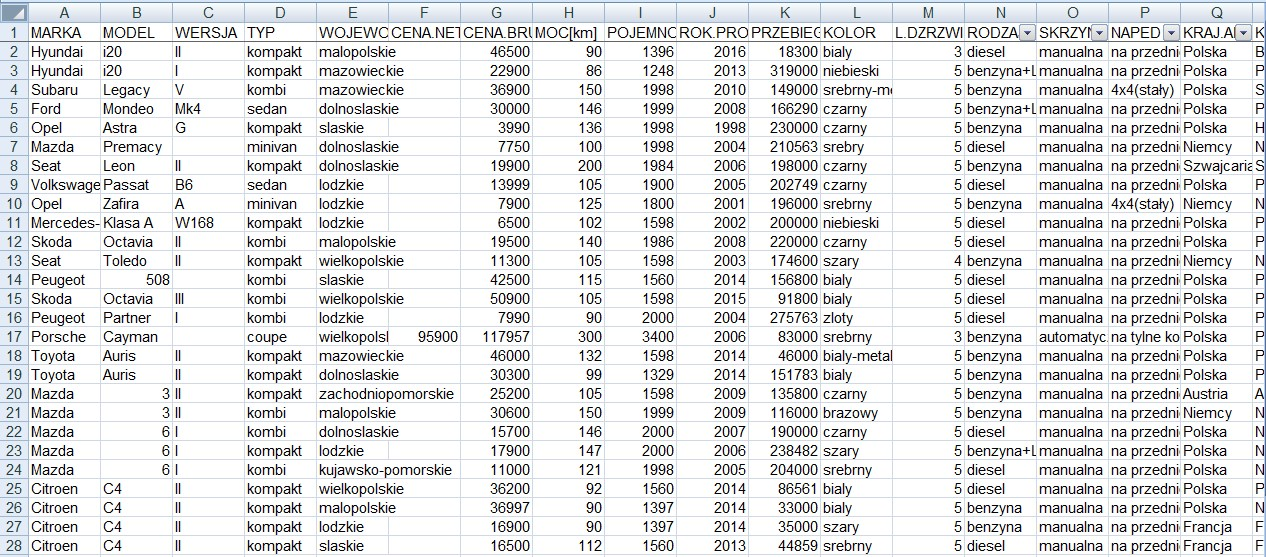
\includegraphics[width=1\textwidth]{zbior2}
\caption{Podgląd stworzonego zbioru}
\label{fig:obrazek1}
\end{figure}


\subsubsection{Użyte zmienne}
\noindent

W stworzonym zbiorze danych znajduje się 29 atrybutów, opisujących 61 różnych rekordów. Wśród zebranych danych można wyróżnić zarówno zmienne jakościowe, jak i ilościowe. 

Zmiennymi jakościowymi są atrybuty: MARKA, MODEL, WERSJA, TYP, WOJEWODZTWO, KOLOR, RODZAJ.PALIWA, SKRZYNIA.BIEGOW, NAPED, 
\newline
KRAJ.AKTUALNEJ.REJESTRACJI, KRAJ.POCHODZENIA, STAN, ABS,
\newline
STATUS.POJAZDU.SPROWADZONEGO, PIERWSZY.WLASCICIEL, KTO.SPRZEDAJE, SERWISOWANY, KOMPUTER.POKLADOWY, ESP, KLIMATYZACJA, BEZWYPADKOWY, USZKODZONY.
\newline
Wśród zmiennych jakościowych można wyróżnić zmienne porządkowe, nominalne oraz binarne. W stworzonym zbiorze danych zmiennymi binarnymi są atrybuty: PIERWSZY.WLASCICIEL, SERWISOWANY, ABS, KOMPUTER.POKLADOWY, ESP, BEZWYPADKOWY, USZKODZONY. Pozostałe atrybuty są zmiennymi nominalnymi.%%%czy aby na pewno zmienne binarne? 

Zmiennymi ilościowymi są atrybuty: CENA.[PLN].NETTO, CENA.[PLN].BRUTTO, MOC, POJEMNOSC.SKOKOWA[cm3], ROK.PRODUKCJI, PRZEBIEG[km], L.DRZWI. 
\newline
Wśród zmiennych ilościowych można wyróżnić zmienne skokowe oraz dyskretne. W stworzonym zbiorze danych, zmiennymi skokowymi są: MOC, POJEMNOŚĆ.SKOKOWA[cm3], ROK.PRODUKCJI, PRZEBIEG, L.DRZWI. Z kolei atrybuty: CENA.[PLN].NETTO, CENA.[PLN].BRUTTO są zmiennymi ciągłymi. 
%czy zmienne porządkowe nie powinny być zaliczane do zmiennych ilościowych?
%l.drzwi powinna zostać zaliczona do zmiennych porządkowych 

%wrzucic screen pogladowy do tych danych


\bibliographystyle{plain}
\bibliography{plik_z_bibliografia}





%% F1 F11 F1 F1
\end{document}
